\documentclass{scrreprt}
\usepackage{listings}
\usepackage{underscore}
\usepackage[bookmarks=true]{hyperref}
\usepackage[utf8]{inputenc}
\usepackage[spanish]{babel}
\usepackage{array}
\usepackage{graphicx}
\usepackage{placeins}
\usepackage{tabularx,ragged2e}
\newcolumntype{L}{>{\RaggedRight}X}
\newcolumntype{P}[1]{>{\centering\arraybackslash}p{#1}}
\hypersetup{
    bookmarks=false,    % show bookmarks bar?
    pdftitle={Especificación de Requerimientos},   
    pdfauthor={Kevin Valle Soledispa},                     
    pdfsubject={TeX and LaTeX},                       
    pdfkeywords={TeX, LaTeX, graphics, images}, 
    colorlinks=true,       
    linkcolor=blue,
    citecolor=black,       
    filecolor=black,        
    urlcolor=purple,        
    linktoc=page            
}%
\def\myversion{1.2 }
\date{}
%\title
\usepackage{hyperref}
\begin{document}

\begin{center}
    \rule{16cm}{4pt}\vskip1cm
    \begin{bfseries}
        \Huge{ESPECIFICACIÓN DE\\ REQUERIMIENTOS}\\
        \vspace{1.5cm}
        $Stocktaking$\\
        \vspace{1.5cm}
        \begin{figure}[!htpb]
            \centerline{
\includegraphics[scale=.68]{images/logo_espol.png}}
        \end{figure}    
        \LARGE{Versión \myversion}\\
        \vspace{1.5cm}
        Integrantes - Grupo 2:\\
        1. Loor Barragan Carlos Alejandro\\
        2. Auria Perez Eliana Lilibeth\\
        3. Muñoz Carranza Viviana Stephania\\
        4. Valle Soledispa Kevin Paul\\
        \vspace{1.5cm}
        $15/11/22$\\
    \end{bfseries}
\end{center}

\tableofcontents
\listoffigures
\listoftables

\begin{table}[h]
    \setlength\extrarowheight{2pt}
    \caption{Revisión Histórica\strut}
    \begin{tabularx}{\textwidth}{|l|l|p{5cm}|l|} 
        \hline
	    Día & Versión & Descripción & Autor\\
        \hline
	    Octubre 19, 2022 & 1.0 & Resumen ejecutivo, stakeholders, objetivos, alcance y módulos del sistema inicial. & Equipo Stocktaking\\
        \hline
	    Octubre 25, 2022 & 1.1 & Ajustes a nuevos requerimientos del cliente con base a las revisiones hechas por la gerencia de la empresa. & Equipo Stocktaking\\
        \hline
        Noviembre 13, 2022 & 1.2 & Historias de usuarios, clasificación de requerimientos no funcionales y prototipo del sistema & Equipo Stocktaking\\
        \hline
    \end{tabularx}
\end{table}

\chapter{Manejo del Proyecto}

\section{Propósito del Proyecto}
\subsection{Precedentes y Esfuerzos Previos}
Importadora Andina es una empresa que brinda servicio y asesoramiento en venta, post venta y mantenimiento en el ámbito automotriz a nivel nacional. Actualmente cuenta con 14 sucursales, 8 tecnicentros y 6 puntos de venta mayorista repartidos en 11 provincias alrededor del país, lo cual genera una gran cantidad de información que solo puede ser accedida por los empleados dentro de la red privada de la empresa. Esto supone un inconveniente en el flujo de trabajo ya que la información no está disponible para ellos cuando están fuera del alcance de la red. Por esta razón, surgió la necesidad de crear una plataforma web con un módulo móvil que permita al personal de Importadora Andina realizar consultas por medio de internet sin importar en qué lugar se encuentren y tener la información requerida para registrar y monitorear los movimientos de los bienes tangibles de la empresa.

\subsection{Metas}
Como equipo se buscará construir una plataforma web que gestione el inventario de manera eficiente bajo estándares de diseño y desarrollo establecidos por la empresa, además de permitir el manejo y gestión del inventario en el cual los usuarios puedan consultar reportes de documentos contables y comerciales mediante el acceso a la base de datos de la empresa. Simultáneamente, se construirá un aplicativo móvil en el cual se podrá escanear productos mediante sus códigos QR para así obtener sus datos y generar un reporte que se podrá descargar.
Al ayudar con el registro y consulta de sus productos se optimizará el desempeño de sus operaciones a nivel nacional y local creando un flujo de trabajo más eficiente. 

\section{Stakeholders}
\subsection{Gerencia de la Empresa}
La gerencia de la empresa provee de financiamiento al proyecto e instrucciones generales, además de que el sistema les va a permitir revisar el estado del inventario de su empresa desde cualquier lado, permitiéndoles un control y supervisión más precisos del inventario y las operaciones de la empresa. 

\subsection{Departamento Tecnológico de la Empresa}
Este departamento brinda la información de los sistemas actualmente desplegados en la empresa y de las posibilidades de interacción con ellos, además de colaborar con nosotros de manera activa en el desarrollo de la plataforma, por último estos van a ser los encargados de darle mantenimiento futuro a la misma, por lo tanto van a tener que estar informados del funcionamiento de esta y tener acceso y comprensión del backend para poder solucionar problemas o añadir nuevas funcionalidades en un futuro.\\
Las responsabilidades de este stakeholder son:
\begin{itemize}
    \item Aceptar o rechazar cambios en el software
    \item Guiar el proceso de levantamiento de requerimientos 
    \item Pruebas de usuarios del sistema
    \item Entrega de Retroalimentación acerca del estado de la plataforma web y móvil
\end{itemize}

\subsection{Departamento de Ventas}
Estos son unos de los usuarios principales, ya que ellos van a poder visualizar saldos de inventario actual, el Kardex de mercadería, lista de precios y existencia, listados de facturas con entregas pendientes, consultar comprobantes electrónicos, el listado de guías de remisión y órdenes de despacho. Por lo tanto, su comprensión del funcionamiento de la plataforma es necesaria y vital que los vuelve parte integral del desarrollo. 

\subsection{Empleados de Bodega}
Son los encargados de actualizar los valores de inventario, por lo tanto, deben de ser capaces de interactuar con la plataforma para realizar cambios a la existencia de productos, añadir o remover, etc. También son los encargados del escaneo de las baterías que salen de bodega a manos de los consumidores. 

\subsection{Departamento de Contabilidad}
Su función será revisar de manera rápida las facturas que consideren de su interés y también que los documentos contables estén correctamente estructurados. 

\subsection{Departamento de Auditoría}
Ellos van a utilizar la plataforma cuando se realice el proceso para consistencia de saldos de inventarios por agencia, por lo tanto, deben de ser capaces de utilizar el producto para realizar esta tarea y esto implica acceso a casi toda la información que va a estar disponible en el mismo, por ende, su feedback también va a ser importante en el desarrollo de la aplicación. 

\subsection{Departamento de Entrega}
Usarán el software para visualizar el listado de órdenes de despacho, por lo tanto, también serán usuarios activos de la plataforma y sus opiniones deben ser consideradas en el desarrollo. 

\section{Restricciones Mandatorias}
Estas se basan en el sistema que posee la empresa:
\begin{enumerate}
    \item El sistema requiere que los usuarios ingresen por medio de una identificación de usuario, contraseña y agencia para su respectiva validación.
    \item El registro de usuario ya existe y se realiza desde el sistema ERP de la empresa.
    \item El nivel de acceso de cada usuario ya está previamente definido en la base de datos.
    \item Los filtros de búsquedas se deben activar/visualizar dependiendo de los permisos de usuario.
    \item La empresa proveerá los formatos de consultas y/o reportes a generar.
    \item Las descargas realizadas en la sección de comprobantes electrónicos serán solo en formato PDF, así como el reporte generado en el aplicativo móvil.
    \item El sistema debe interactuar de manera directa con una base de datos en SQLServer, la cual ya ha sido creada por la empresa y ya tiene definidas todas las transacciones que van a ser usadas.
\end{enumerate}

\section{Terminología}

\begin{table}[h]
    \setlength\extrarowheight{2pt}
    \caption{Glosario de Términos\strut}
    \begin{tabularx}{\textwidth}{|l|L|}
            \hline
    	    \textbf {Terminología} & {Significado}\\
            \hline
    	    \textbf {ERP} & Es un sistema que ayuda a automatizar y administrar los procesos empresariales de las distintas áreas de la empresa.\\
            \hline
    	    \textbf Línea de mercadería & Es un grupo de artículos, los cuales están relacionados por funcionalidades o características comunes que los vuelven parte de una misma clasificación de mercadería.\\
            \hline
            \textbf Kardex de mercadería & Es un documento que utiliza la empresa para administrar la mercadería que tiene disponible en el inventario. El formato suele ser dependiente de cada empresa.\\
            \hline
            \textbf Orden de despacho & Es un documento que ampara el traslado de los productos de un lugar a otro.\\
            \hline
            \textbf Tecnicentro & Un centro de asistencia técnica que es propiedad de la empresa, en el cual se venden productos y se ofrecen servicios relacionados al mantenimiento de equipos mecánicos.\\
            \hline
            \textbf Comprobantes electrónicos & Tipo de factura entregado en formato electrónico.\\
            \hline
            \textbf Documento de entrega & Es un documento propio de la empresa, cuya funcionalidad es documentar los códigos y la información individual de la mercadería que fue entregada en una compra, usando como método de referencia el código de la factura de la compra en cuestión.\\
            \hline
    \end{tabularx}
\end{table}



\begin{table}[h]
    \setlength\extrarowheight{2pt}
    \caption{Glosario de Términos 2\strut}
    \begin{tabularx}{\textwidth}{|l|L|}
        \hline
        Guías de remisión & Son documentos mercantiles que registran los traslados de mercadería o las entregas de pedidos.\\
        \hline
        Ordenes de despacho & Es un documento usado en el traslado de mercaderías para respaldar la entrega efectiva de los productos.\\
        \hline
        Hoja de despacho & Son documentos mercantiles que registran la entrega de mercadería o pedidos.\\
        \hline
        Hoja de ruta de despacho & Es un documento que registra la ruta que se va a tomar para cumplir con la orden de despacho, además de contener los datos del conductor y la placa del vehículo.\\
        \hline
        Rango secuencial del documento & A cada documento se le asigna un número de secuencia que sirve como identificador.\\
        \hline
    \end{tabularx}
\end{table}

\begin{table}[h]
    \setlength\extrarowheight{2pt}
    \caption{Glosario de Acrónimos\strut}
    \begin{tabularx}{\textwidth}{|l|L|}
        \hline
    	 Acrónimos & Significado\\
        \hline
        ERP & Enterprise Resource Planning (Planificación de recursos empresariales).\\
        \hline
       QR & Quick Response.\\
        \hline
    \end{tabularx}
\end{table}

\chapter{Requerimientos Funcionales}

\section{Alcance del Proyecto}
Se desarrollarán versiones semi funcionales de una página web responsiva y su componente móvil. Los programas estarán listos para ser entregados cuando cuenten con un diseño disponible para la visualización del cliente y cuando permitan usos básicos de aspectos del inventario.\\

Funcionalidades de la página web responsiva:
\begin{itemize}
    \item Saldos de inventario actual.
    \item Kardex de mercadería.
    \item Lista de precios y existencia.
    \item Listado de facturas con entregas pendientes.
    \item Listado de guías de remisión y órdenes de despacho.
    \item Mayor de mercaderías.
    \item Proceso para consistencia de los saldos de inventarios por agencia.
\end{itemize}
\\

Además, el  componente móvil tendrá como funcionalidad:
\begin{itemize}
    \item Escaneo de los códigos QR presentes en la mercadería que sale de bodega con motivo de venta.
\end{itemize}
\\

Los programas funcionarán únicamente dentro de la empresa Importadora Andina en computadores con sistema operativo Windows y se entregarán aplicaciones móviles solo para dispositivos Android, excluyendo la plataforma de IOS. La plataforma deberá interactuar de manera directa con la base de datos preexistente del cliente, la cual funciona en SQL Server. Se usará la información de la base de datos para validar el acceso de los usuarios además de mostrar información acerca del inventario y facturaciones de la empresa ya que la creación y registro de estos datos son responsabilidades de otros sistemas de la empresa. 
Actualmente se conocen 7 diferentes roles de usuario que harán uso de las plataformas descritas anteriormente, los departamentos de gerencia, tecnología, ventas, contabilidad y auditoría tendrán acceso al sitio web realizando el mismo flujo de trabajo, sin embargo, los filtros que estos puedan aplicar a la información y el acceso que tengan a ella dependerán de su nivel de autorización dentro de la organización.
Los departamentos de entregas y empleados de bodega tendrán acceso a la aplicación móvil con el mismo flujo de trabajo. La relación de roles, actividades, departamentos y tecnología se detalla en los casos de uso descritos de acuerdo a cada funcionalidad (ver Anexo A).

\section{Historias de Usuario}

\begin{table}[h]
    \setlength\extrarowheight{2pt}
    \caption{Identificador 01\strut}
    \begin{tabularx}{\textwidth}{|l|L|} 
        \hline
        \textbf{ID} & 01  \\
        \hline
        \textbf{Título} & Inicio de Sesión \\
        \hline
        \textbf{Actor} & Miembro de la Empresa \\
        \hline
        \textbf{Historia de Usuario} & Como miembro de la empresa, quiero iniciar sesión en el aplicativo usando nombre de usuario, contraseña y código de local para acceder al sistema.\\ 
        \hline
        \multicolumn{2}{|l|}{\textbf{MoSCoW}: Must} \\
        \hline
    \end{tabularx}
\end{table}

\begin{table}[h]
    \setlength\extrarowheight{2pt}
    \caption{Identificador 02\strut}
    \begin{tabularx}{\textwidth}{|l|L|} 
        \hline
        \textbf{ID} & 02  \\
        \hline
        \textbf{Título} & Consulta de Kardex \\
        \hline
        \textbf{Actor} & Personal de Bodega \\
        \hline
        \textbf{Historia de Usuario} & Como personal de bodega, quiero consultar el Kardex de mercadería para administrar la mercancía que la empresa tiene en su inventario.\\ 
        \hline
        \multicolumn{2}{|l|}{\textbf{MoSCoW}: Must} \\
        \hline
    \end{tabularx}
\end{table}

\begin{table}[h]
    \setlength\extrarowheight{2pt}
    \caption{Identificador 03\strut}
    \begin{tabularx}{\textwidth}{|l|L|} 
        \hline
        \textbf{ID} & 03  \\
        \hline
        \textbf{Título} & Visualización de Kardex \\
        \hline
        \textbf{Actor} & Personal de Bodega \\
        \hline
        \textbf{Historia de Usuario} & Como personal de bodega, quiero visualizar los Kardex de mercadería filtrados por local, zona, código de artículo, línea de artículo y rango de fecha para facilitar la administración de la mercancía que la empresa tiene en su inventario.\\ 
        \hline
        \multicolumn{2}{|l|}{\textbf{MoSCoW}: Must} \\
        \hline
        \multicolumn{2}{|l|}{\textbf{Dependiente de}: 02} \\
        \hline
    \end{tabularx}
\end{table}

\begin{table}[h]
    \setlength\extrarowheight{2pt}
    \caption{Identificador 04\strut}
    \begin{tabularx}{\textwidth}{|l|L|} 
        \hline
        \textbf{ID} & 04  \\
        \hline
        \textbf{Título} & Captura de Datos por Códigos QR \\
        \hline
        \textbf{Actor} & Personal de Bodega \\
        \hline
        \textbf{Historia de Usuario} & Como personal de bodega, quiero capturar el código único de identificación de la mercadería obtenido mediante el escaneo del código QR propio de cada producto para generar un documento de entrega de la mercadería despachada en cada orden.\\
        \hline
        \multicolumn{2}{|l|}{\textbf{MoSCoW}: Must} \\
        \hline
    \end{tabularx}
\end{table}

\begin{table}[h]
    \setlength\extrarowheight{2pt}
    \caption{Identificador 05\strut}
    \begin{tabularx}{\textwidth}{|l|L|} 
        \hline
        \textbf{ID} & 05  \\
        \hline
        \textbf{Título} & Generar Reporte por Código QR \\
        \hline
        \textbf{Actor} & Personal de Bodega \\
        \hline
        \textbf{Historia de Usuario} & Como personal de bodega, quiero que la plataforma genere un documento de entrega al escanear un Código QR para tener un récord de los productos despachados en cada orden.\\ 
        \hline
        \multicolumn{2}{|l|}{\textbf{MoSCoW}: Must} \\
        \hline
        \multicolumn{2}{|l|}{\textbf{Dependiente de}: 04} \\
        \hline
    \end{tabularx}
\end{table}

\begin{table}[h]
    \setlength\extrarowheight{2pt}
    \caption{Identificador 06\strut}
    \begin{tabularx}{\textwidth}{|l|L|} 
        \hline
        \textbf{ID} & 06\\
        \hline
        \textbf{Título} & Consulta del Reporte Generado por Código QR \\
        \hline
        \textbf{Actor} & Personal de Bodega \\
        \hline
        \textbf{Historia de Usuario} & Como personal de bodega, quiero consultar el documento de entrega correspondiente a un producto para visualizar la mercadería entregada con respecto a una factura.\\ 
        \hline
        \multicolumn{2}{|l|}{\textbf{MoSCoW}: Should} \\
        \hline
        \multicolumn{2}{|l|}{\textbf{Dependiente de}: 05} \\
        \hline
    \end{tabularx}
\end{table}

\begin{table}[h]
    \setlength\extrarowheight{2pt}
    \caption{Identificador 07\strut}
    \begin{tabularx}{\textwidth}{|l|L|} 
        \hline
        \textbf{ID} & 07 \\
        \hline
        \textbf{Título} & Imprimir Reporte Generado por Código QR \\
        \hline
        \textbf{Actor} & Personal de Bodega \\
        \hline
        \textbf{Historia de Usuario} & Como personal de bodega, quiero imprimir el documento de entrega correspondiente a un producto para visualizar la mercadería entregada con respecto a una factura en un documento físico.\\ 
        \hline
        \multicolumn{2}{|l|}{\textbf{MoSCoW}: Must} \\
        \hline
        \multicolumn{2}{|l|}{\textbf{Dependiente de}: 06} \\
        \hline
    \end{tabularx}
\end{table}

\begin{table}[h]
    \setlength\extrarowheight{2pt}
    \caption{Identificador 08\strut}
    \begin{tabularx}{\textwidth}{|l|L|} 
        \hline
        \textbf{ID} & 08  \\
        \hline
        \textbf{Título} & Consulta de Comprobantes Electrónicos \\
        \hline
        \textbf{Actor} & Vendedor \\
        \hline
        \textbf{Historia de Usuario} & Como vendedor, quiero consultar los comprobantes electrónicos emitidos para revisar las ordenes entregadas, su costo y los productos relacionados.\\ 
        \hline
        \multicolumn{2}{|l|}{\textbf{MoSCoW}: Must} \\
        \hline
    \end{tabularx}
\end{table}

\begin{table}[h]
    \setlength\extrarowheight{2pt}
    \caption{Identificador 09 \strut}
    \begin{tabularx}{\textwidth}{|l|L|} 
        \hline
        \textbf{ID} & 09 \\
        \hline
        \textbf{Título} & Visualizar Comprobantes Electrónicos \\
        \hline
        \textbf{Actor} & Vendedor \\
        \hline
        \textbf{Historia de Usuario} & Como vendedor, quiero visualizar los comprobantes electrónicos emitidos filtrados por establecimiento, período de emisión, cliente, tipo de documento, estado de documento (activo e inactivo) y estado de envío a email (enviado o sin enviar) para facilitar la búsqueda de comprobantes.\\ 
        \hline
        \multicolumn{2}{|l|}{\textbf{MoSCoW}: Must} \\
        \hline
        \multicolumn{2}{|l|}{\textbf{Dependiente de}: 08} \\
        \hline
    \end{tabularx}
\end{table}

\begin{table}[h]
    \setlength\extrarowheight{2pt}
    \caption{Identificador 10 \strut}
    \begin{tabularx}{\textwidth}{|l|L|} 
        \hline
        \textbf{ID} & 10 \\
        \hline
        \textbf{Título} & Visualizar el Listado de las Guías de Remisión   \\
        \hline
        \textbf{Actor} & Personal de Bodega \\
        \hline
        \textbf{Historia de Usuario} & Como personal de bodega, quiero visualizar el listado de las guías de remisión para consultar acerca del traslado de mercadería desde un lugar a otro.\\ 
        \hline
        \multicolumn{2}{|l|}{\textbf{MoSCoW}: Must} \\
        \hline
    \end{tabularx}
\end{table}

\begin{table}[h]
    \setlength\extrarowheight{2pt}
    \caption{Identificador 11 \strut}
    \begin{tabularx}{\textwidth}{|l|L|} 
        \hline
        \textbf{ID} & 11 \\
        \hline
        \textbf{Título} & Filtrar Listado de las Guías de Remisión    \\
        \hline
        \textbf{Actor} & Personal de Bodega \\
        \hline
        \textbf{Historia de Usuario} & Como personal de bodega, quiero visualizar el listado de las guías de remisión filtrado por locales a nivel nacional, local o zona, período de emisión y estado de las guías de remisión (activo o inactivo) para facilitar las consultas acerca del traslado de mercadería desde un lugar a otro.\\ 
        \hline
        \multicolumn{2}{|l|}{\textbf{MoSCoW}: Must} \\
        \hline
        \multicolumn{2}{|l|}{\textbf{Dependiente de}: 10} \\
        \hline
    \end{tabularx}
\end{table}

\begin{table}[h]
    \setlength\extrarowheight{2pt}
    \caption{Identificador 12 \strut}
    \begin{tabularx}{\textwidth}{|l|L|} 
        \hline
        \textbf{ID} & 12 \\
        \hline
        \textbf{Título} & Visualizar Listado de Facturas con Entregas Pendientes \\
        \hline
        \textbf{Actor} & Personal de Bodega \\
        \hline
        \textbf{Historia de Usuario} & Como personal de bodega, quiero visualizar un listado de las facturas con entregas pendientes para revisar los compromisos de entrega que tiene la empresa con sus clientes. \\ 
        \hline
        \multicolumn{2}{|l|}{\textbf{MoSCoW}: Must} \\
        \hline
    \end{tabularx}
\end{table}

\begin{table}[h]
    \setlength\extrarowheight{2pt}
    \caption{Identificador 13 \strut}
    \begin{tabularx}{\textwidth}{|l|L|} 
        \hline
        \textbf{ID} & 13 \\
        \hline
        \textbf{Título} & Visualizar Facturas con Entregas Pendientes \\
        \hline
        \textbf{Actor} & Personal de Bodega \\
        \hline
        \textbf{Historia de Usuario} & Como personal de bodega, quiero visualizar las facturas con entregas pendientes que muestre el número del local, código del documento, código y nombre del cliente y artículo para obtener información detallada de cada entrega. \\ 
        \hline
        \multicolumn{2}{|l|}{\textbf{MoSCoW}: Must} \\
        \hline
        \multicolumn{2}{|l|}{\textbf{Dependiente de}: 12} \\
        \hline
    \end{tabularx}
\end{table}

\begin{table}[h]
    \setlength\extrarowheight{2pt}
    \caption{Identificador 14 \strut}
    \begin{tabularx}{\textwidth}{|l|L|} 
        \hline
        \textbf{ID} & 14 \\
        \hline
        \textbf{Título} & Filtrar Búsqueda de Facturas con Entregas Pendientes \\
        \hline
        \textbf{Actor} & Personal de Bodega \\
        \hline
        \textbf{Historia de Usuario} & Como personal de bodega, quiero filtrar las facturas con entregas pendientes por rango de fecha, por código y/o nombre del cliente y 3 distintos niveles de ubicación: nacional, zonal y local para facilitar la búsqueda de facturas en específico.\\ 
        \hline
        \multicolumn{2}{|l|}{\textbf{MoSCoW}: Must} \\
        \hline
        \multicolumn{2}{|l|}{\textbf{Dependiente}: 13} \\
        \hline
    \end{tabularx}
\end{table}

\begin{table}[h]
    \setlength\extrarowheight{2pt}
    \caption{Identificador 15 \strut}
    \begin{tabularx}{\textwidth}{|l|L|} 
        \hline
        \textbf{ID} & 15 \\
        \hline
        \textbf{Título} & Visualizar el Listado de Ordenes de Despacho \\
        \hline
        \textbf{Actor} & Personal de Bodega \\
        \hline
        \textbf{Historia de Usuario} & Como personal de bodega, quiero visualizar un listado de órdenes de despacho para autorizar la salida de mercadería correspondiente.\\ 
        \hline
        \multicolumn{2}{|l|}{\textbf{MoSCoW}: Must} \\
        \hline
    \end{tabularx}
\end{table}

\begin{table}[h]
    \setlength\extrarowheight{2pt}
    \caption{Identificador 16 \strut}
    \begin{tabularx}{\textwidth}{|l|L|} 
        \hline
        \textbf{ID} & 16 \\
        \hline
        \textbf{Título} & Visualizar Detalles del Listado de Ordenes de Despacho \\
        \hline
        \textbf{Actor} & Personal de Bodega \\
        \hline
        \textbf{Historia de Usuario} & Como personal de bodega, quiero que el listado de órdenes de despacho muestre el local de emisión de la orden, el número de la orden, la fecha de su emisión, el nombre del conductor y su número de cedula, las placas del vehículo, además de la fecha de inicio y fin del traslado para poder visualizar esta información sin descargar los documentos. \\ 
        \hline
        \multicolumn{2}{|l|}{\textbf{MoSCoW}: Must} \\
        \hline
        \multicolumn{2}{|l|}{\textbf{Dependiente de}: 15} \\
        \hline
    \end{tabularx}
\end{table}

\begin{table}[h]
    \setlength\extrarowheight{2pt}
    \caption{Identificador 17 \strut}
    \begin{tabularx}{\textwidth}{|l|L|} 
        \hline
        \textbf{ID} & 17 \\
        \hline
        \textbf{Título} & Descargar Orden de Despacho en PDF \\
        \hline
        \textbf{Actor} & Personal de Bodega \\
        \hline
        \textbf{Historia de Usuario} & Como personal de bodega, quiero que el listado de órdenes de despacho tenga la opción de descargar una orden de despacho en PDF para compartir el documento con personas ajenas a la plataforma.  \\ 
        \hline
        \multicolumn{2}{|l|}{\textbf{Dependiente de}: 16} \\
        \hline
    \end{tabularx}
\end{table}

\begin{table}[h]
    \setlength\extrarowheight{2pt}
    \caption{Identificador 18 \strut}
    \begin{tabularx}{\textwidth}{|l|L|} 
        \hline
        \textbf{ID} & 18 \\
        \hline
        \textbf{Título} & Descargar Hoja de Despacho en PDF \\
        \hline
        \textbf{Actor} & Personal de Bodega \\
        \hline
        \textbf{Historia de Usuario} & Como personal de bodega, quiero que el listado de órdenes de despacho tenga la opción de descargar una hoja de despacho en PDF para compartir el documento con personas ajenas a la plataforma. \\ 
        \hline
        \multicolumn{2}{|l|}{\textbf{MoSCoW}: Should} \\
        \hline
        \multicolumn{2}{|l|}{\textbf{Dependiente de}: 16} \\
        \hline
    \end{tabularx}
\end{table}

\begin{table}[h]
    \setlength\extrarowheight{2pt}
    \caption{Identificador 19 \strut}
    \begin{tabularx}{\textwidth}{|l|L|} 
        \hline
        \textbf{ID} & 19 \\
        \hline
        \textbf{Título} & Descargar Hoja de Ruta de Despacho en PDF \\
        \hline
        \textbf{Actor} & Personal de Bodega \\
        \hline
        \textbf{Historia de Usuario} & Como personal de bodega, quiero que el listado de órdenes de despacho tenga la opción de descargar una hoja de ruta de despacho en PDF para compartir el documento con personas ajenas a la plataforma.\\ 
        \hline
        \multicolumn{2}{|l|}{\textbf{MoSCoW}: Should} \\
        \hline
        \multicolumn{2}{|l|}{\textbf{Dependiente de}: 16} \\
        \hline
    \end{tabularx}
\end{table}

\begin{table}[h]
    \setlength\extrarowheight{2pt}
    \caption{Identificador  20 \strut}
    \begin{tabularx}{\textwidth}{|l|L|} 
        \hline
        \textbf{ID} & 09 - 5 \\
        \hline
        \textbf{Título} & Filtrar Búsqueda de Listado de Ordenes de Despacho \\
        \hline
        \textbf{Actor} & Personal de Bodega \\
        \hline
        \textbf{Historia de Usuario} & Como personal de bodega, quiero visualizar un listado de órdenes de despacho filtrado por local, zona, periodo de emisión y rango secuencial del documento para facilitar el proceso de autorización de salida de mercadería correspondiente.\\ 
        \hline
        \multicolumn{2}{|l|}{\textbf{MoSCoW}: Must} \\
        \hline
        \multicolumn{2}{|l|}{\textbf{Dependiente de}: 15} \\
        \hline
    \end{tabularx}
\end{table}

\begin{table}[h]
    \setlength\extrarowheight{2pt}
    \caption{Identificador 21 \strut}
    \begin{tabularx}{\textwidth}{|l|L|} 
        \hline
        \textbf{ID} & 21 \\
        \hline
        \textbf{Título} & Visualizar Stock de Producto \\
        \hline
        \textbf{Actor} & Miembro del Equipo de Ventas \\
        \hline
        \textbf{Historia de Usuario} & Como miembro del equipo de ventas quiero visualizar la lista de productos en stock para conocer los productos disponibles para la venta.\\ 
        \hline
        \multicolumn{2}{|l|}{\textbf{MoSCoW}: Must} \\
        \hline
    \end{tabularx}
\end{table}

\begin{table}[h]
    \setlength\extrarowheight{2pt}
    \caption{Identificador 21 \strut}
    \begin{tabularx}{\textwidth}{|l|L|} 
        \hline
        \textbf{ID} & 21 \\
        \hline
        \textbf{Título} & Visualizar Mayor de Mercadería \\
        \hline
        \textbf{Actor} & Personal de Departamento Contable \\
        \hline
        \textbf{Historia de Usuario} & Como personal del departamento contable, quiero consultar el mayor de mercadería para conocer el estado de la sucursal.\\ 
        \hline
        \multicolumn{2}{|l|}{\textbf{MoSCoW}: Must} \\
        \hline
    \end{tabularx}
\end{table}

\begin{table}[h]
    \setlength\extrarowheight{2pt}
    \caption{Identificador 22\strut}
    \begin{tabularx}{\textwidth}{|l|L|} 
        \hline
        \textbf{ID} &  22 \\
        \hline
        \textbf{Título} & Filtrar Búsqueda de Mayor de Mercadería \\
        \hline
        \textbf{Actor} & Personal de Departamento Contable \\
        \hline
        \textbf{Historia de Usuario} & Como personal del departamento contable, quiero visualizar el mayor de mercaderías filtrados locales a nivel local o zonal, código de artículo, línea de artículo yrango de fecha para conocer el movimiento de mercadería.\\ 
        \hline
        \multicolumn{2}{|l|}{\textbf{MoSCoW}: Must} \\
        \hline
        \multicolumn{2}{|l|}{\textbf{Dependiente de}: 21} \\
        \hline
    \end{tabularx}
\end{table}

\chapter{Requerimientos No Funcionales}

\section{Requerimientos de Eficiencia}

\begin{enumerate}


    \item El tiempo medio de respuesta de una consulta de documento administrativo (Kardex, mayor de mercadería, guía de remisión, comprobante electrónico, orden de despacho y factura de entrega pendiente) es de 15 segundos. 
    \begin{enumerate}
        \item \textbf{Validación}: Prueba medible\\
           Se realizarán 50 pruebas de consulta y se recolectarán los tiempos en los que fue resuelta la petición, se promediaran los datos y se verificará que la media sea menor a 15 segundos.
        \item \textbf{MoSCoW}: Must
    \end{enumerate}
    
    \item El tiempo máximo de respuesta de una consulta de datos administrativo (Kardex, mayor de mercadería, guía de remisión, comprobante electrónico, orden de despacho y factura de entrega pendiente) es de 20 segundos.  
    \begin{enumerate}
        \item \textbf{Validación}: Simulación\\
        Se realizará 50 pruebas de consulta y se recolectara los tiempos en los que fue resuelta la petición, asegurando que ninguno de estos tome más de 20 segundos.
        \item \textbf{MoSCoW}: Must
    \end{enumerate}
    
    \item El sistema web debe soportar de 4 a 10 usuarios que estén realizando consultas de documentos (Kardex, mayor de mercadería, guía de remisión, comprobante electrónico, orden de despacho y factura de entrega pendiente) simultáneamente.
    \begin{enumerate}
        \item \textbf{Validación}: Simulación\\
        Se conectarán 10 personas de manera simultánea durante 20 minutos y se controlará que el sistema no falle más del 1\% del tiempo de las pruebas.
        \item \textbf{MoSCoW}: Must
    \end{enumerate}
    
    \item La aplicación móvil debe soportar de 3 a 5 empleados de bodega ubicados en un mismo local que estén interactuando con el sistema de manera simultánea. 
    \begin{enumerate}
        \item \textbf{Validación}: Simulación\\
        Se conectarán 5 personas de manera simultánea durante 20 minutos y se controlará que el sistema no falle más del 1\% del tiempo.
        \item \textbf{MoSCoW}: Should
    \end{enumerate}
    
    \item La aplicación móvil debe soportar de 20 a 25 empleados de bodega ubicados en diferentes locales a nivel nacional que estén interactuando con el sistema de manera simultánea. 
    \begin{enumerate}
        \item \textbf{Validación}: Simulación\\
        Inicialmente se conectarán 20 usuarios de manera simultánea que eventualmente aumentarán de uno en uno hasta llegar a los 25 usuarios durante 10 minutos y se controlará que el sistema no falle más del 1\% del tiempo de prueba. 
        \item \textbf{MoSCoW}: Must
    \end{enumerate}
    
    \item El tiempo de actualización de la pantalla del sistema debe demorar en promedio de 15 a 20 segundos bajo una conexión a internet con velocidad igual o superior a los 50 megabytes por segundo.
    \begin{enumerate}
        \item \textbf{Validación}: Prueba medible\\
        Se realizarán 50 pruebas de actualización y se recolectarán los tiempos en los que fue resuelta la petición para promediar los datos y verificar que el promedio esté entre los 15 a 20 segundos.
        \item \textbf{MoSCoW}: Must
    \end{enumerate}
    
    \item El tiempo máximo de descarga de un lote de 10 facturas debe ser en promedio de 10 a 25 segundos bajo una conexión a internet con velocidad igual o superior a los 50 megabytes por segundo. 
    \begin{enumerate}
        \item \textbf{Validación}: Prueba medible\\
        Se realizarán 50 pruebas de descarga y se recolectarán los tiempos en los que fue resuelta la petición para promediar los datos y verificar que el promedio esté entre los 10 y 25 segundos.
        \item \textbf{MoSCoW}: Must
    \end{enumerate}
    
\end{enumerate}

\section{Requerimientos de Usabilidad}

\begin{enumerate}


    \item Las horas de capacitación al personal de bodega requeridas para el uso del sistema móvil debe ser de 2 horas máximo en una sola sesión de instrucción.
    \begin{enumerate}
        \item \textbf{Validación}: Prueba medible\\
        Se dará un curso de instrucción cuya duración será de 2 horas a 10 empleados de bodega, que cumplan con dos requisitos: tener 5 años de experiencia laboral en su puesto actual y ser menores de 35 años. Al concluir el curso, ellos deberán ser capaces de escanear el código QR y enlazar el código en cuestión a una factura del sistema. Además, los empleados capacitados contarán con el manual de uso de la aplicación.
        \item \textbf{MoSCoW}: Should
    \end{enumerate}
    
    
    \item El personal de bodega deberá estar adaptado al uso del sistema móvil en 1 semana máximo.
    \begin{enumerate}
        \item \textbf{Validación}: Prueba medible\\
        Se dará un curso de instrucción cuya duración será de 2 horas a 10 empleados de bodega, que cumplan con dos requisitos: tener 5 años de experiencia laboral en su puesto actual y ser menores de 35 años. Al concluir el curso, ellos deberán ser capaces de escanear el código QR y enlazar el código en cuestión a una factura del sistema, sin necesidad de un manual de uso de la aplicación.
        \item \textbf{MoSCoW}: Should
    \end{enumerate}
    
    
\end{enumerate}

\section{Requerimientos de Producto}

\begin{enumerate}
    \item El sistema deberá estar disponible el 99\% del tiempo operacional entre las 5AM a 7PM dentro del año laboral. 
    \begin{enumerate}
        \item \textbf{Validación}: Simulación\\
        Se simulará el sistema activo durante el periodo correspondiente a un año operacional, este deberá estar disponible el 99\% del tiempo. 
        \item \textbf{MoSCoW}: Must
    \end{enumerate}
\end{enumerate}

\section{Requerimientos Organizacionales}
\subsection{Diseño}
\begin{enumerate}
    \item El sistema web debe desarrollarse usando Angular como framework de desarrollo. 
    \item El sistema móvil debe operar bajo el sistema operativo de Android.
\end{enumerate}

\chapter{Información Adicional}

\section{Apéndice A: Casos de Uso}

\begin{figure}[!htpb]
    \centerline{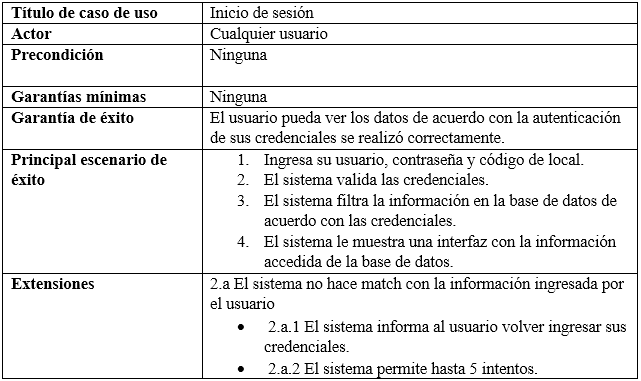
\includegraphics[scale=.50]{images/case_stiff/stuff1.png}}
    \caption{Caso de Uso 1 - Inicio de Sesión.}
    \label{fig}
\end{figure}
\FloatBarrier

\begin{figure}[!htpb]75
    \centerline{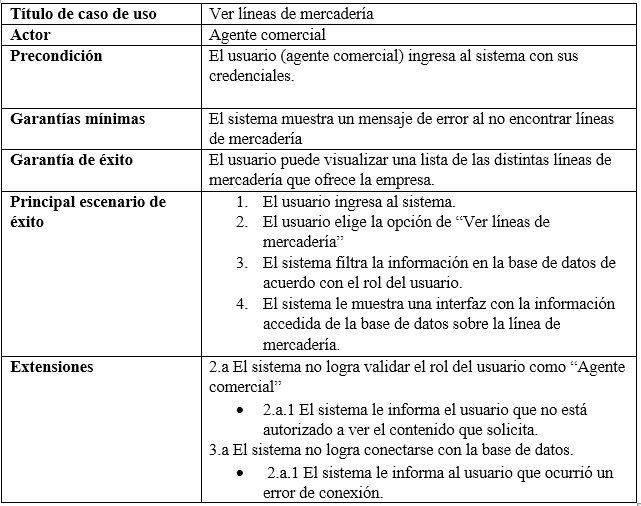
\includegraphics[scale=.50]{images/case_stiff/stuff2.png}}
    \caption{Caso de Uso 2 - Ver Líneas de Mercadería.}
    \label{fig}
\end{figure}
\FloatBarrier

\begin{figure}[!htpb]
    \centerline{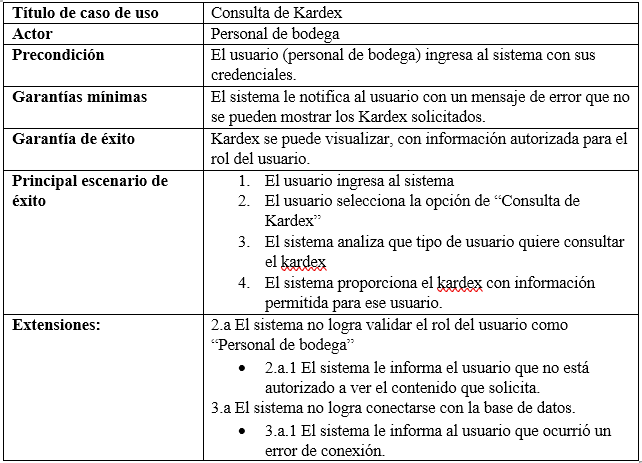
\includegraphics[scale=.75]{images/case_stiff/stuff3.png}}
    \caption{Caso de Uso 3 - Consulta de Kardex.}
    \label{fig}
\end{figure}
\FloatBarrier

\begin{figure}[!htpb]
    \centerline{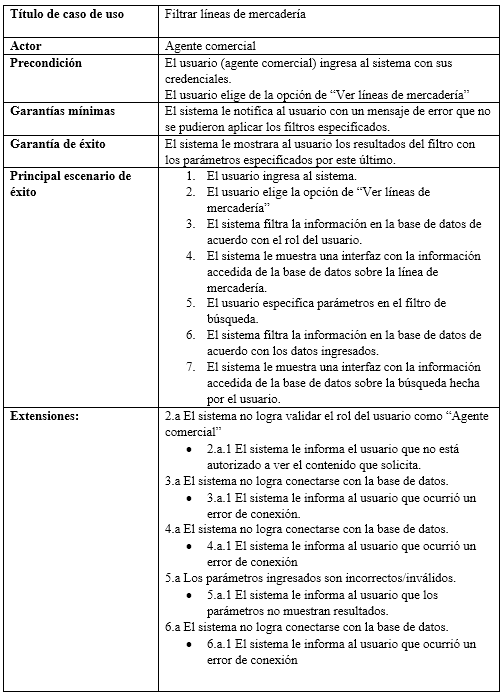
\includegraphics[scale=.75]{images/case_stiff/stuff34.png}}
    \caption{Caso de Uso 4 - Filtrar Línea de Mercadería.}
    \label{fig}
\end{figure}
\FloatBarrier

\begin{figure}[!htpb]
    \centerline{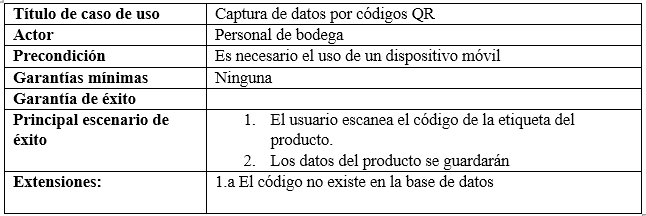
\includegraphics[scale=.75]{images/case_stiff/stuff5.png}}
    \caption{Caso de Uso 5 - Captura de Datos por Códigos QR.}
    \label{fig}
\end{figure}
\FloatBarrier

\begin{figure}[!htpb]
    \centerline{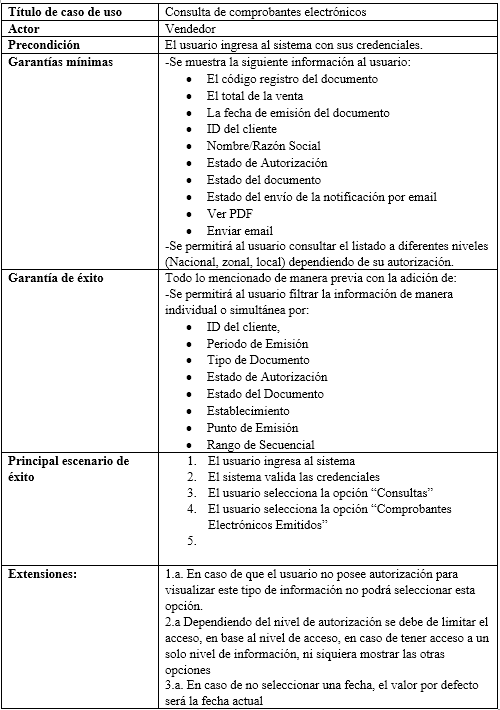
\includegraphics[scale=.75]{images/case_stiff/stuff6.png}}
    \caption{Caso de Uso 6 - Consulta de Comprobantes Electrónicos.}
    \label{fig}
\end{figure}
\FloatBarrier

\begin{figure}[!htpb]
    \centerline{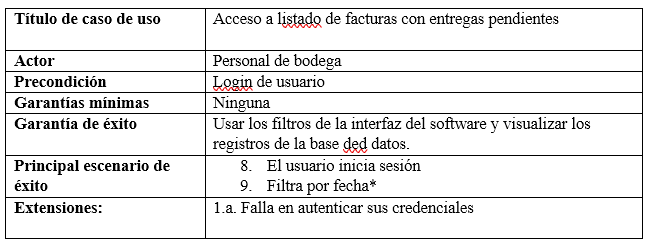
\includegraphics[scale=.75]{images/case_stiff/stuff7.png}}
    \caption{Caso de Uso 7 - Acceso a Listado de Facturas con Entregas Pendientes.}
    \label{fig}
\end{figure}
\FloatBarrier

\begin{figure}[!htpb]
    \centerline{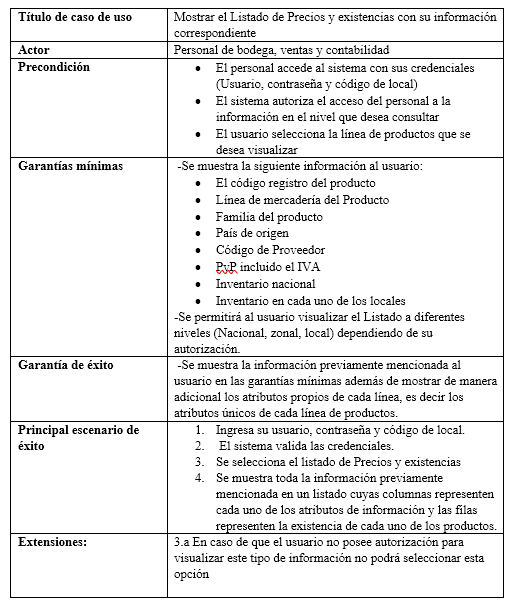
\includegraphics[scale=.75]{images/case_stiff/stuff8.png}}
    \caption{Caso de Uso 8 - Mostrar Listado de Precios y Existencias con su Información Correspondiente.}
    \label{fig}
\end{figure}
\FloatBarrier

\begin{figure}[!htpb]
    \centerline{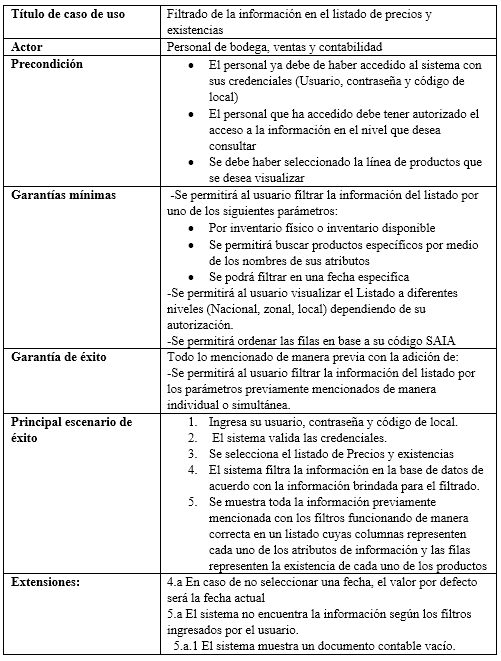
\includegraphics[scale=.90]{images/case_stiff/stuff9.png}}
    \caption{Caso de Uso 9 - Filtrado de Información en Listado de Precios y Existencias.}
    \label{fig}
\end{figure}
\FloatBarrier

\begin{figure}[!htpb]
    \centerline{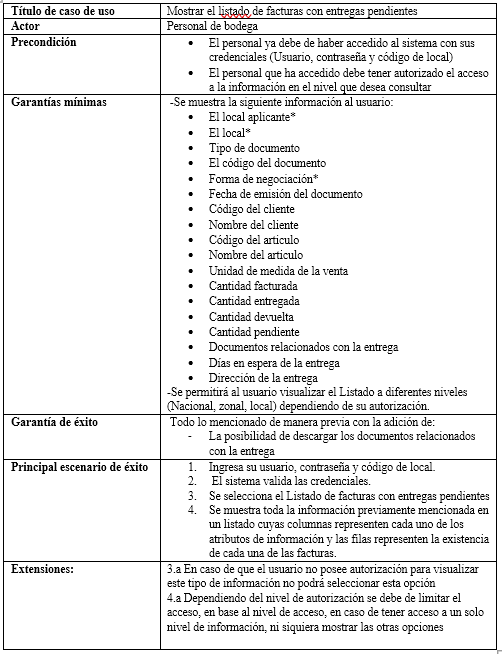
\includegraphics[scale=.90]{images/case_stiff/10.png}}
    \caption{Caso de Uso 10 - Mostrar el Listado de Facturas con Entregas Pendientes.}
    \label{fig}
\end{figure}
\FloatBarrier

\begin{figure}[!htpb]
    \centerline{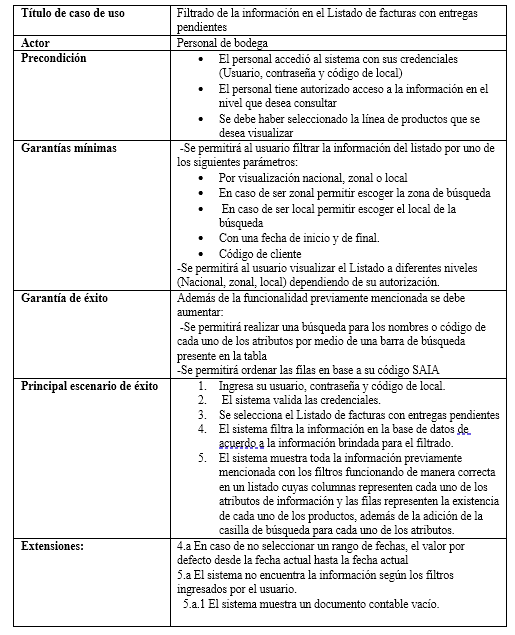
\includegraphics[scale=.90]{images/case_stiff/11.png}}
    \caption{Caso de Uso 11 - Filtrado de Información en Listado de Facturas con Entregas Pendientes.}
    \label{fig}
\end{figure}
\FloatBarrier

\begin{figure}[!htpb]
    \centerline{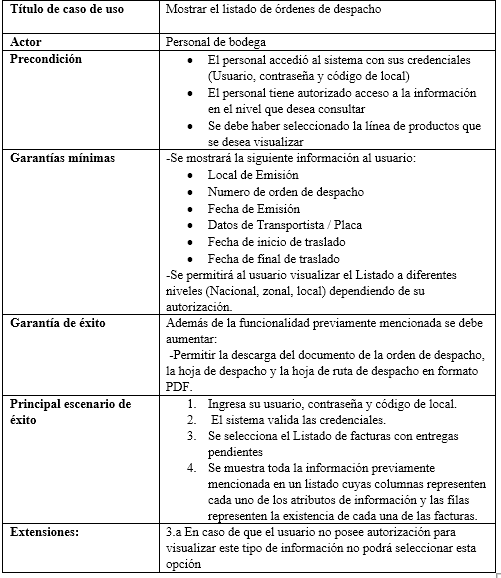
\includegraphics[scale=.75]{images/case_stiff/12.png}}
    \caption{Caso de Uso 12 - Mostrar el Listado de Órdenes de Despacho.}
    \label{fig}
\end{figure}
\FloatBarrier

\begin{figure}[!htpb]
    \centerline{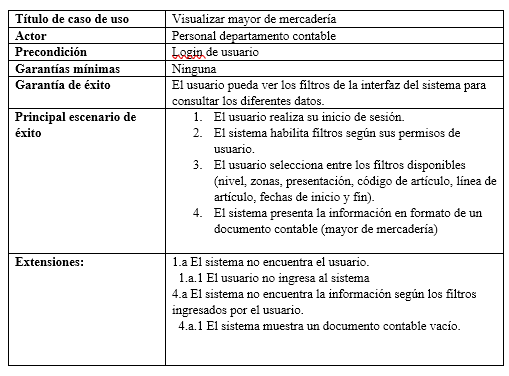
\includegraphics[scale=.90]{images/case_stiff/13.png}}
    \caption{Caso de Uso 13 - Visualizar Mayor de Mercadería.}
    \label{fig}
\end{figure}
\FloatBarrier

\section{Apéndice B: Enlace a Repositorio Público}
https://github.com/ivi-bot/T2-Stocktaking.git\\

\section{Apéndice C: Capturas de Pantalla del Prototipo}


    \subsection{Aplicativo Web}
    \begin{figure}[!htpb]
        \centerline{\includegraphics[scale=.24]{images/prototype/web/Inicio de sesión.png}}
        \caption{Pantalla de Inicio de Sesión.}
        \label{fig}
    \end{figure}
    \FloatBarrier
    

    \begin{figure}[!htpb]
        \centerline{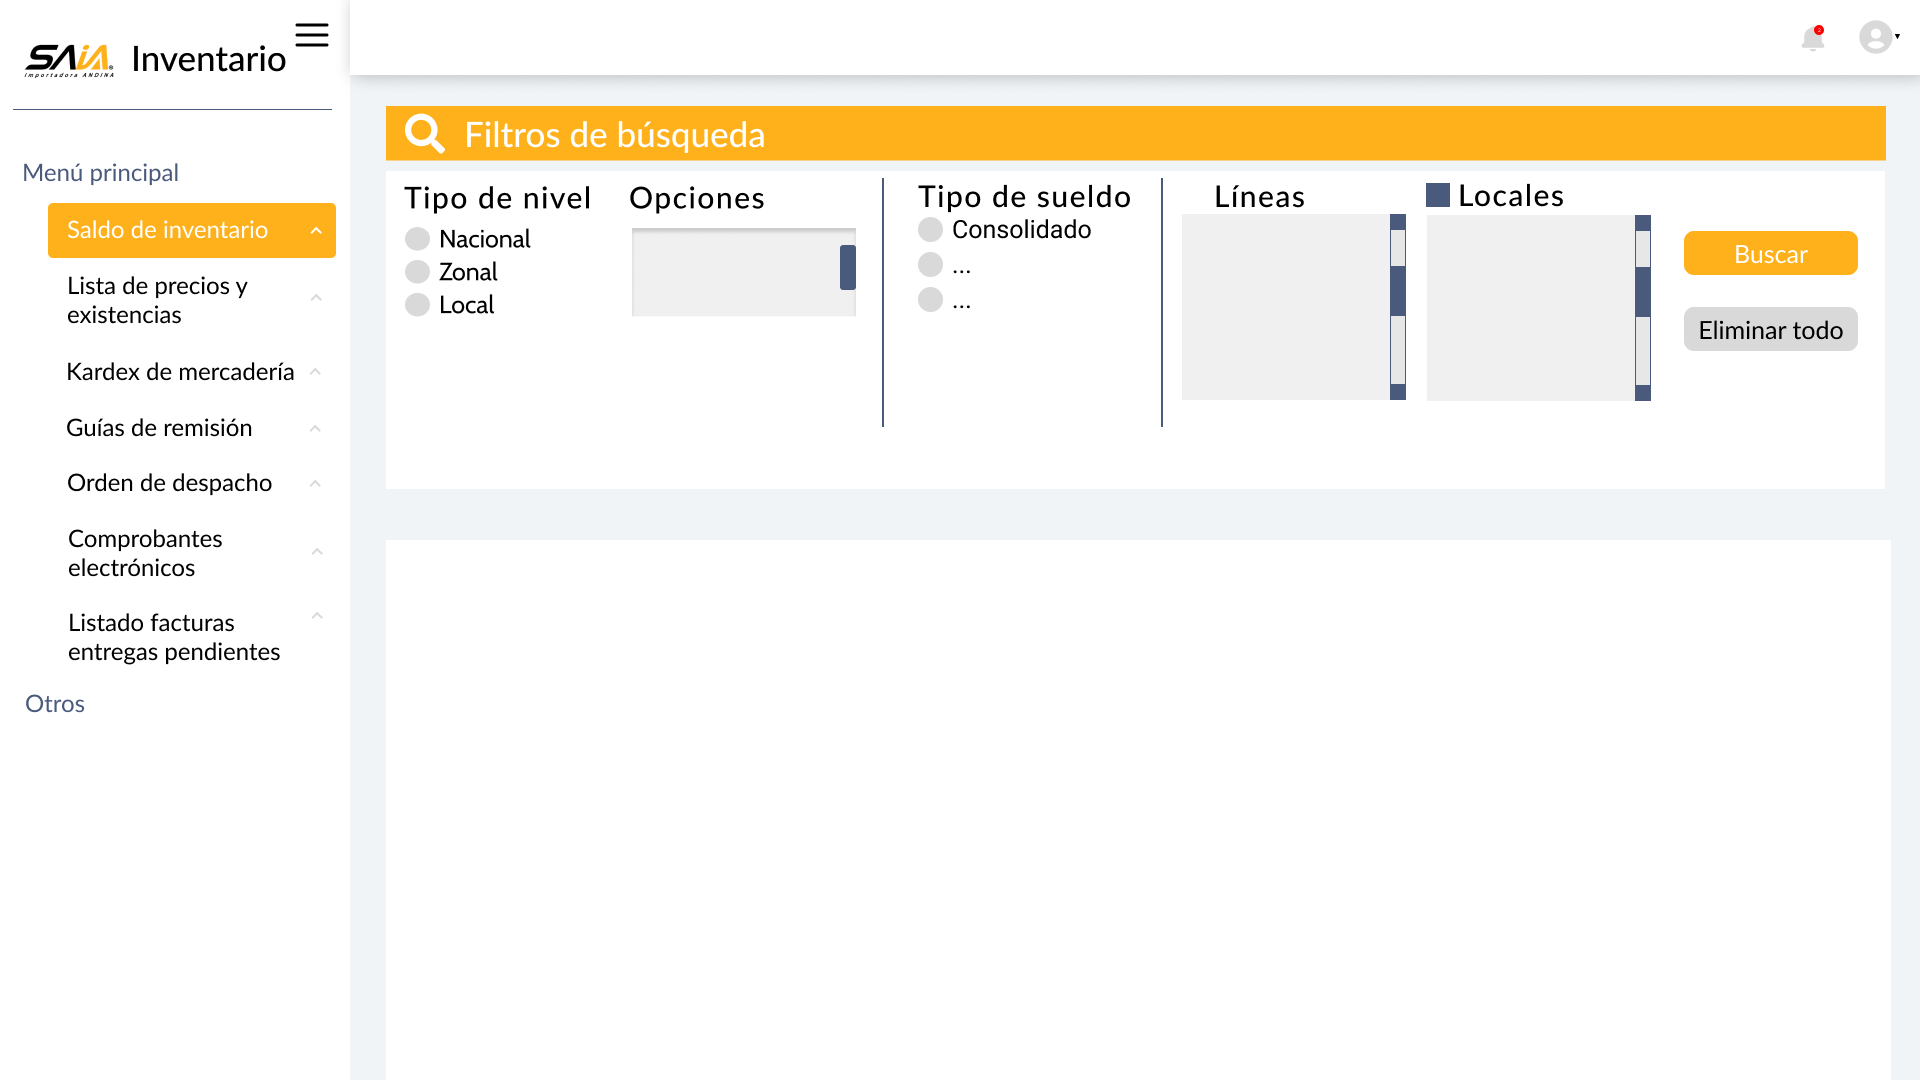
\includegraphics[scale=.24]{images/prototype/web/Saldo de inventario de locales.png}}
        \caption{Apartado de Saldo de inventario.}
        \label{fig}
    \end{figure}
    \FloatBarrier
    \begin{figure}[!htpb]
        \centerline{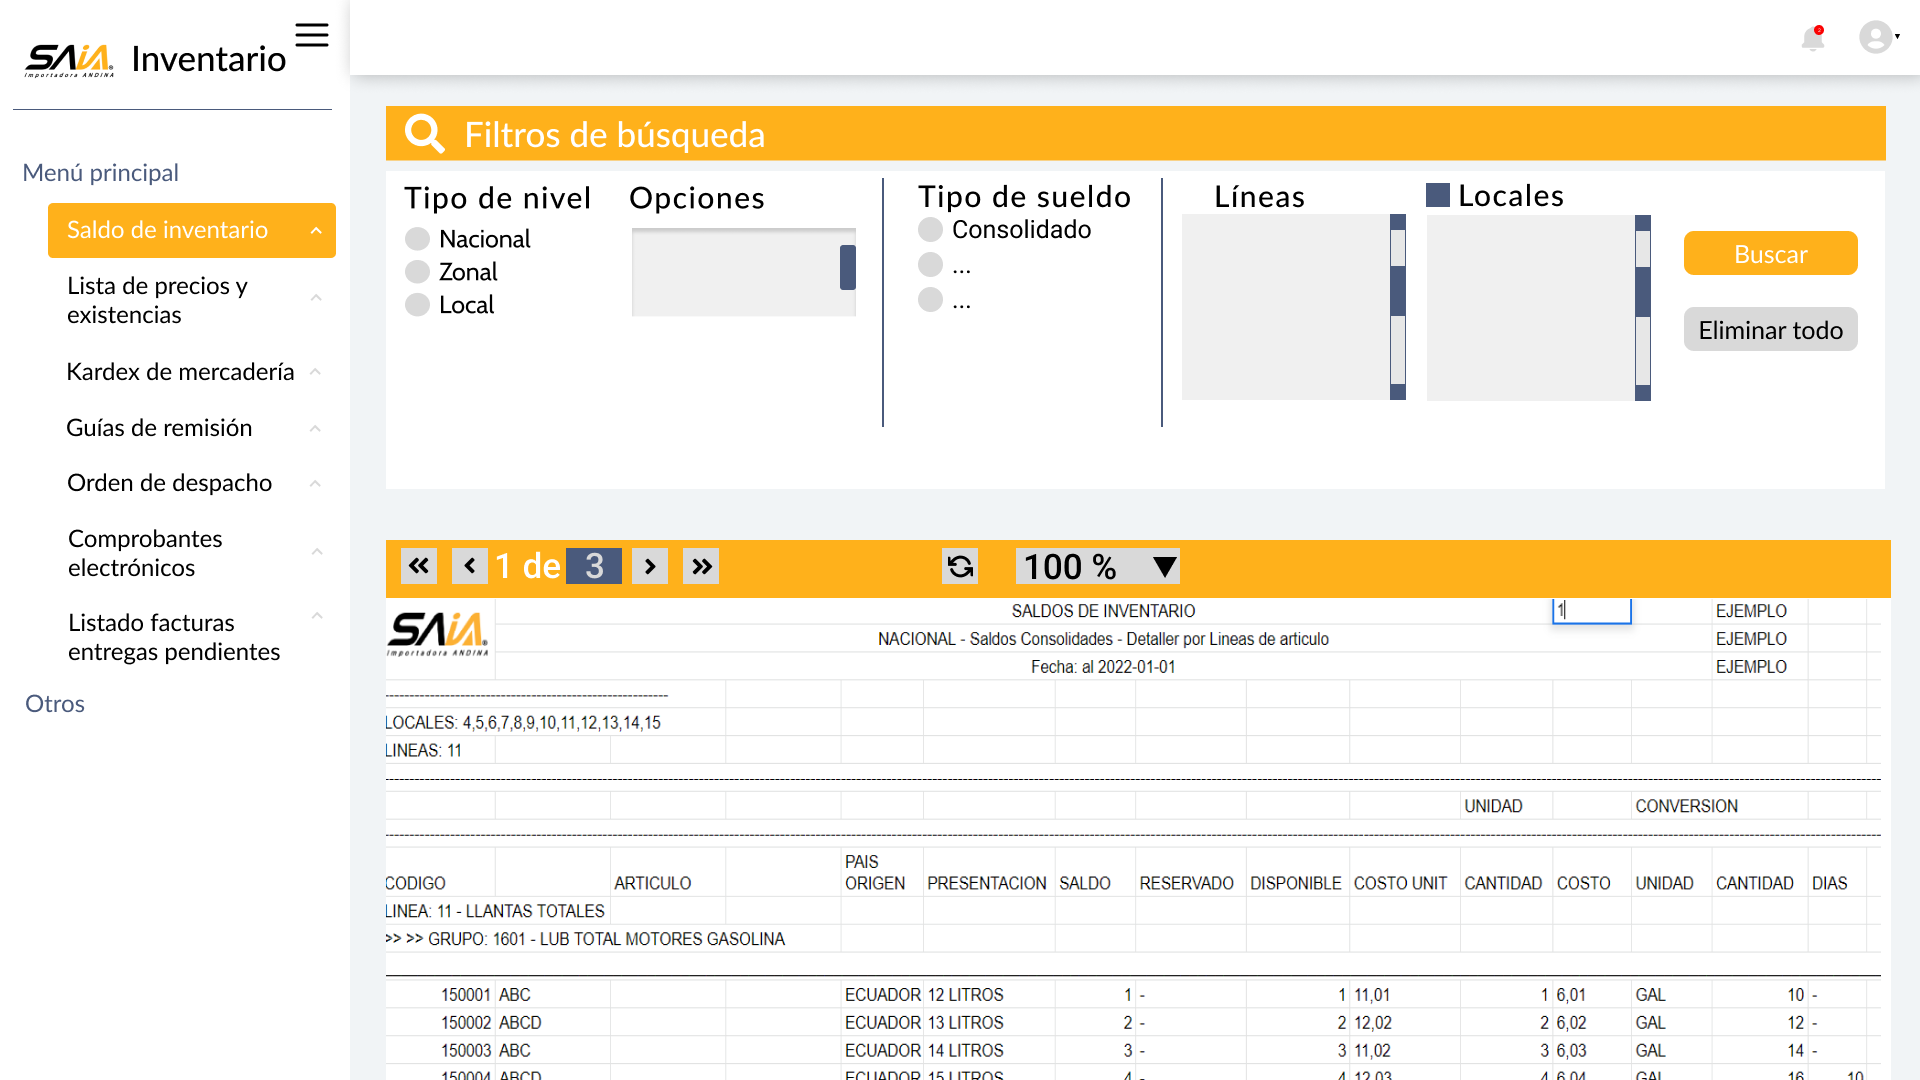
\includegraphics[scale=.24]{images/prototype/web/Saldo de inventario de locales 2.png}}
        \caption{Resultado de filtros de búsqueda aplicados en Saldo de inventario.}
        \label{fig}
    \end{figure}
    
    
    \FloatBarrier
    \begin{figure}[!htpb]
        \centerline{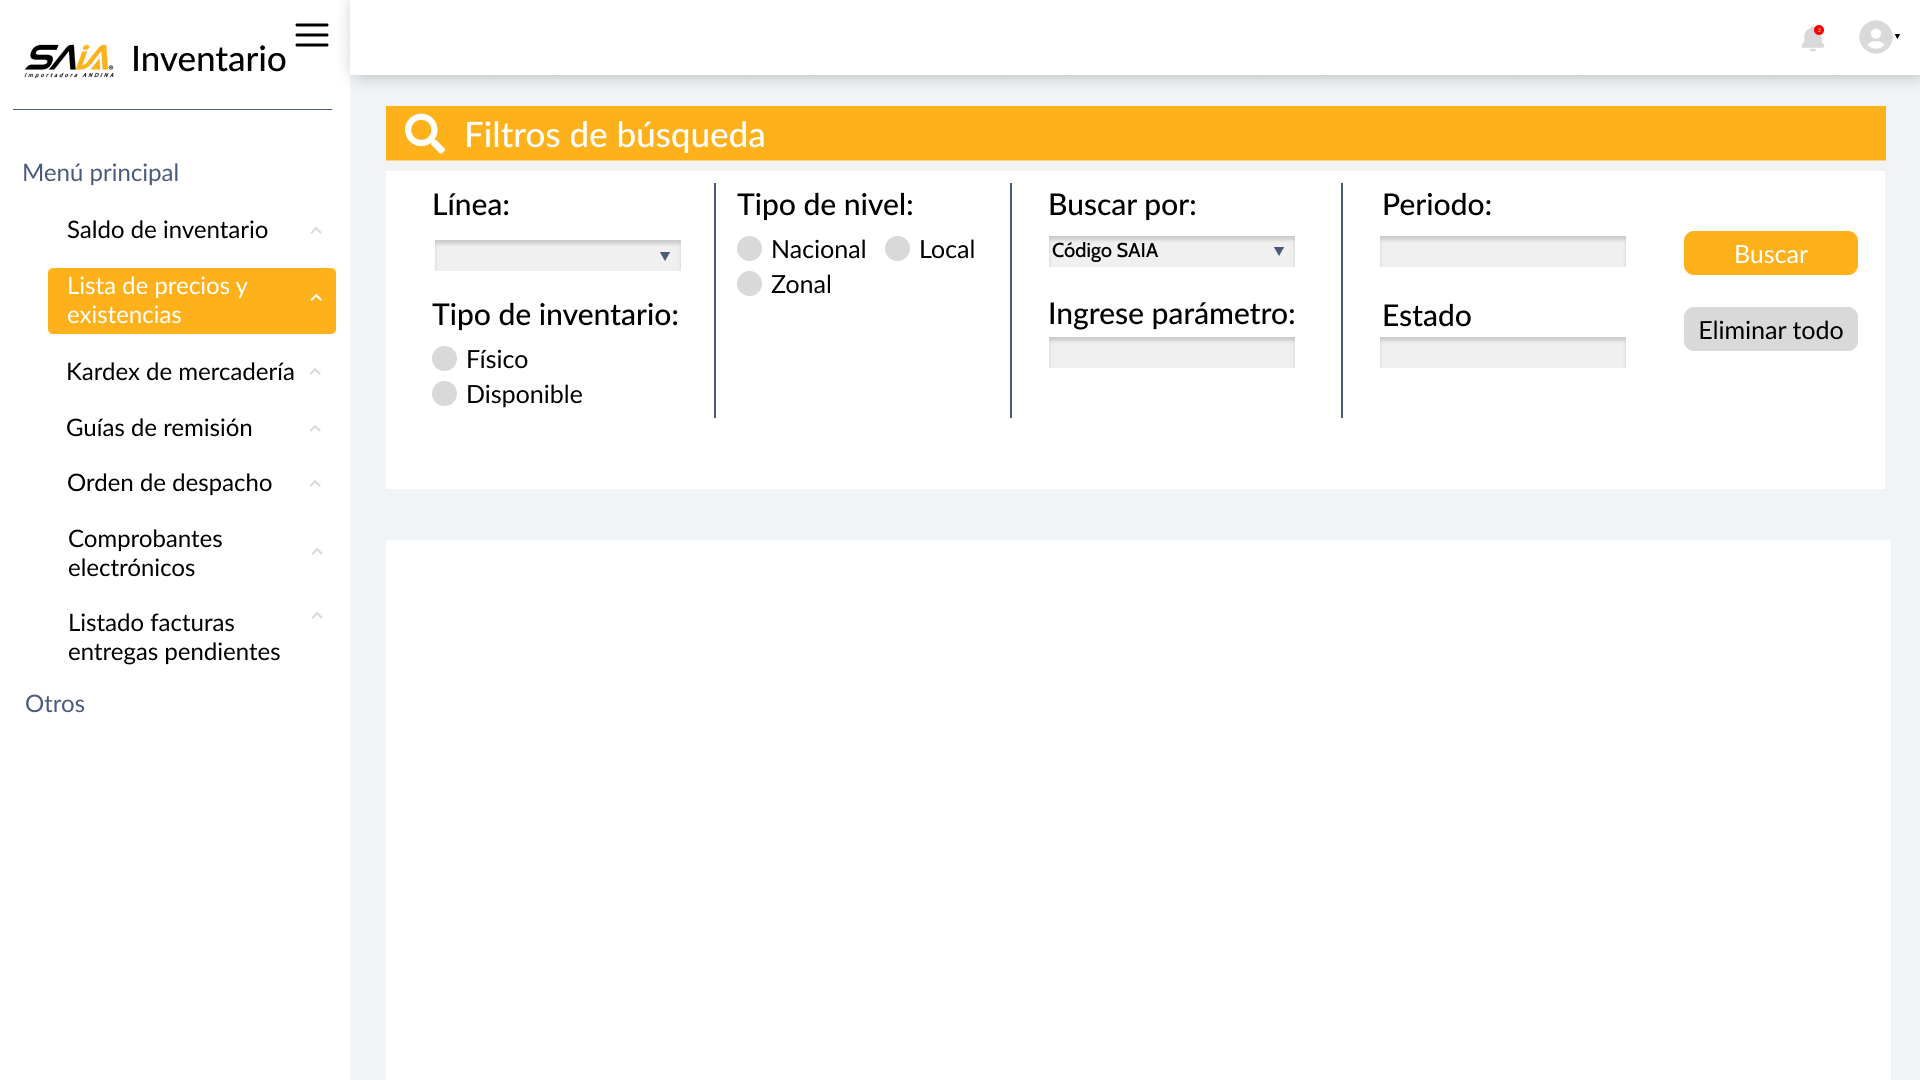
\includegraphics[scale=.24]{images/prototype/web/Saldo de precios y existencias.png}}
        \caption{Apartado de Lista de Precios y Existencias.}
        \label{fig}
    \end{figure}
    \FloatBarrier
    \begin{figure}[!htpb]
        \centerline{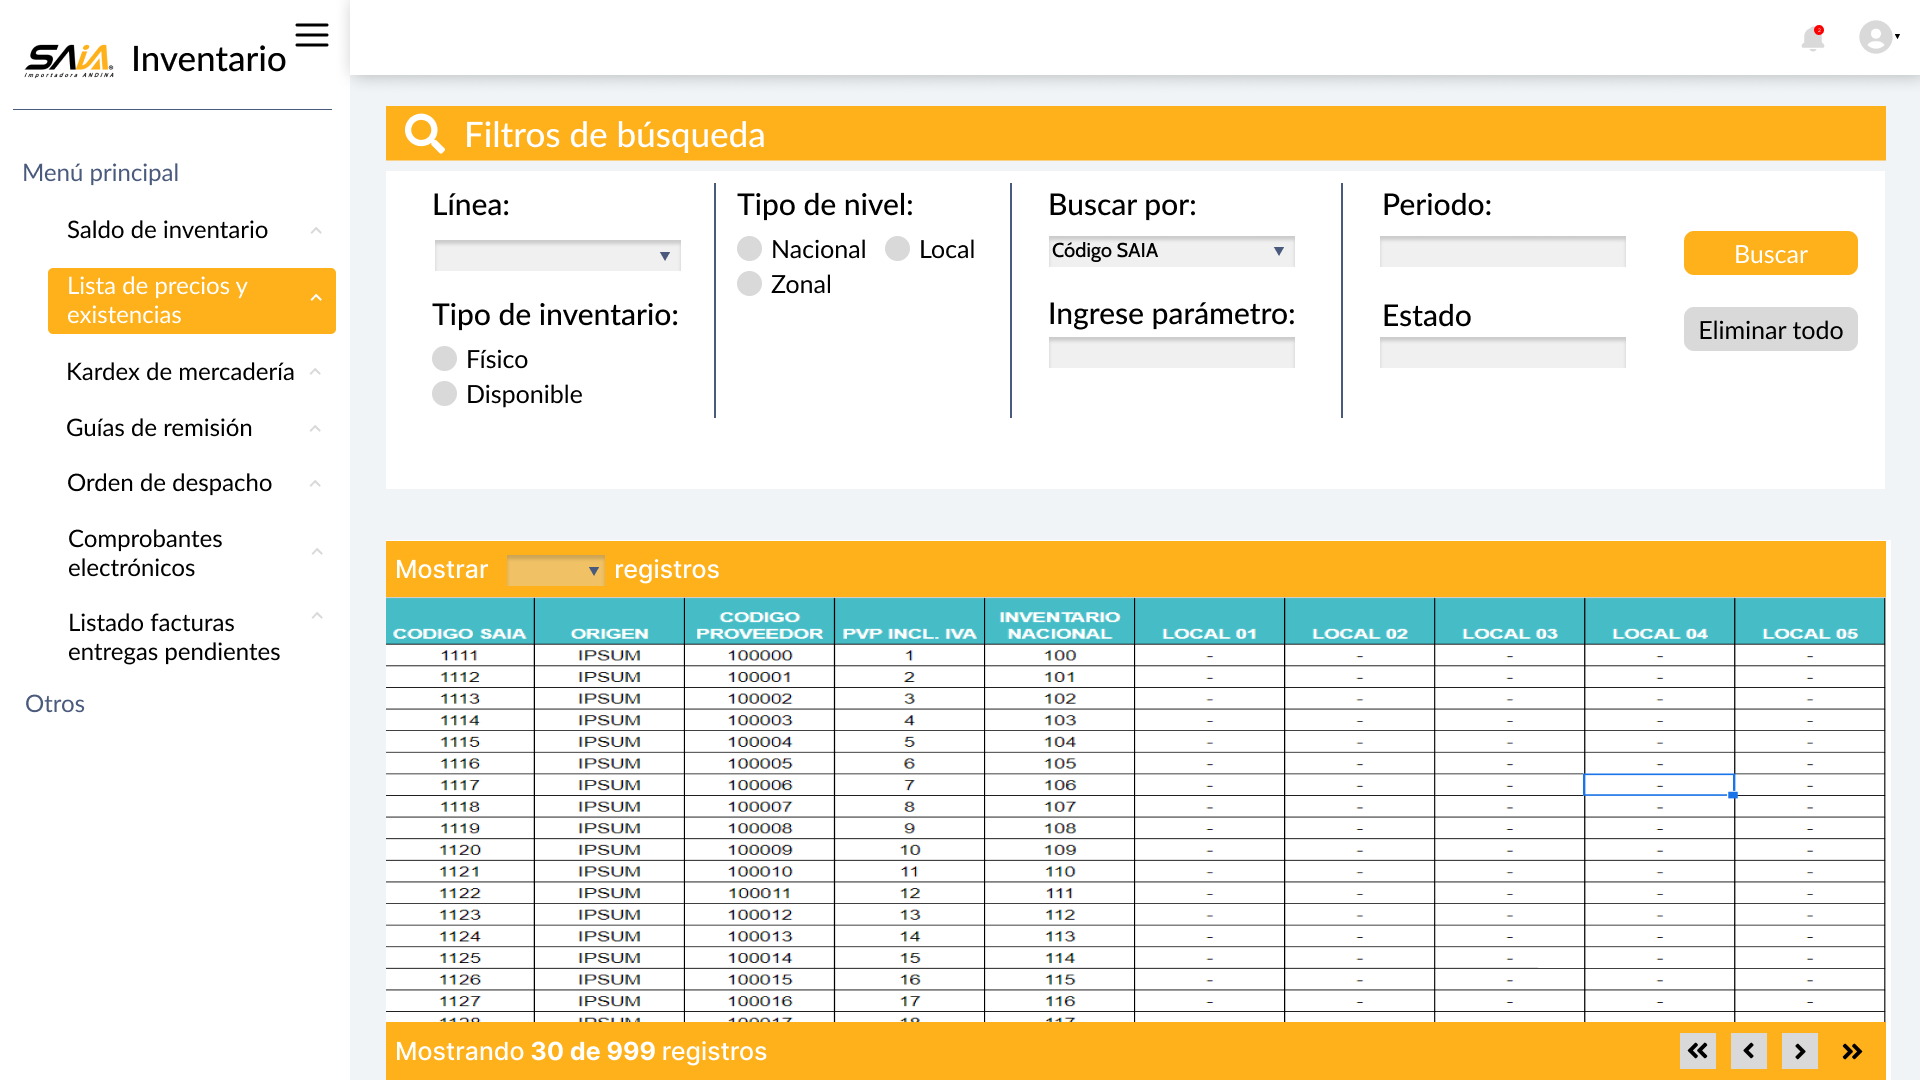
\includegraphics[scale=.20]{images/prototype/web/Saldo de precios y existencias 2.png}}
        \caption{Resultado de filtros de búsqueda aplicados en Lista de Precios y Existencias.}
        \label{fig}
    \end{figure}
    \FloatBarrier
    
    
    \begin{figure}[!htpb]
        \centerline{\includegraphics[scale=.24]{images/prototype/web/Kardex de mercadería.png}}
        \caption{Apartado de Kardex de Mercadería.}
        \label{fig}
    \end{figure}
    \FloatBarrier
    \begin{figure}[!htpb]
        \centerline{\includegraphics[scale=.24]{images/prototype/web/Kardex de mercadería-1.png}}
        \caption{Resultado de filtros de búsqueda aplicados en Kardex de Mercadería.}
        \label{fig}
    \end{figure}
    \FloatBarrier
    

    \begin{figure}[!htpb]
        \centerline{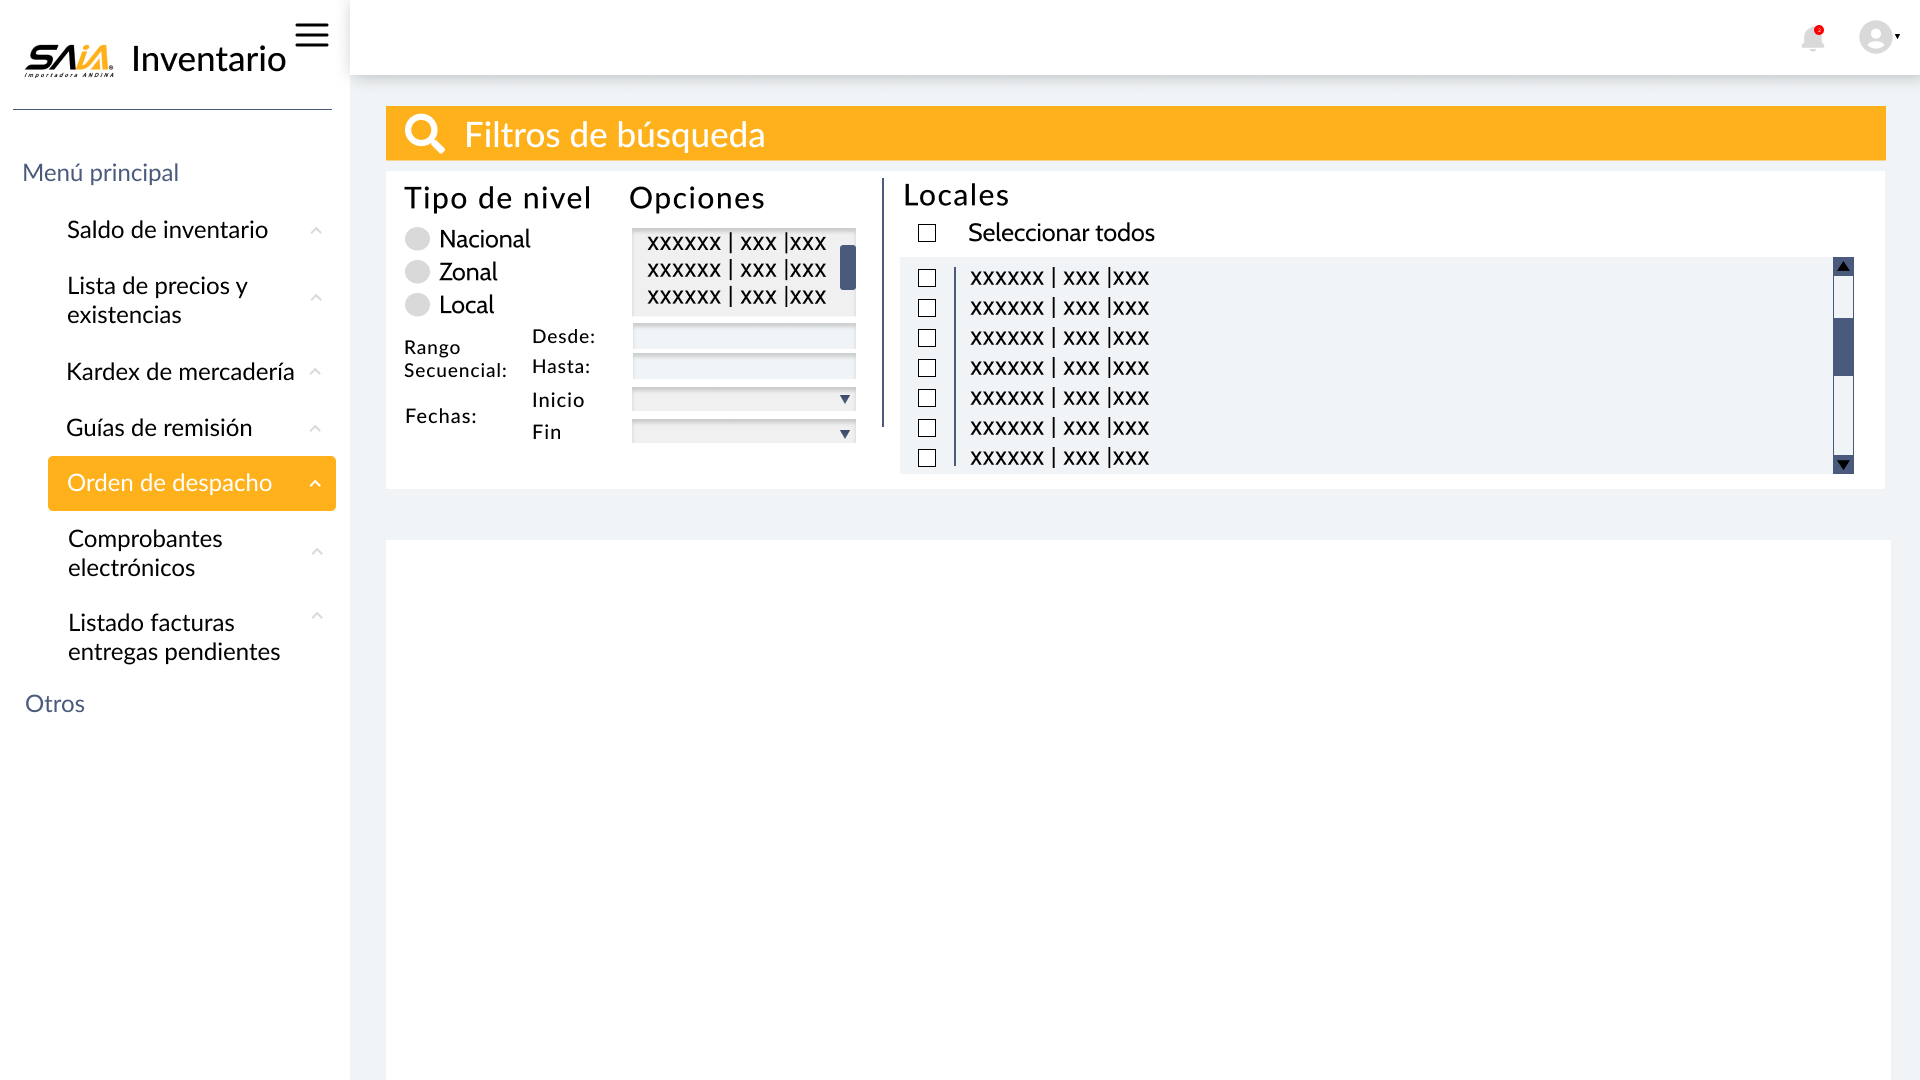
\includegraphics[scale=.22]{images/prototype/web/Ordenes de despacho.png}}
        \caption{Apartado de Ordenes de Despacho.}
        \label{fig}
    \end{figure}
    \FloatBarrier
    \begin{figure}[!htpb]
        \centerline{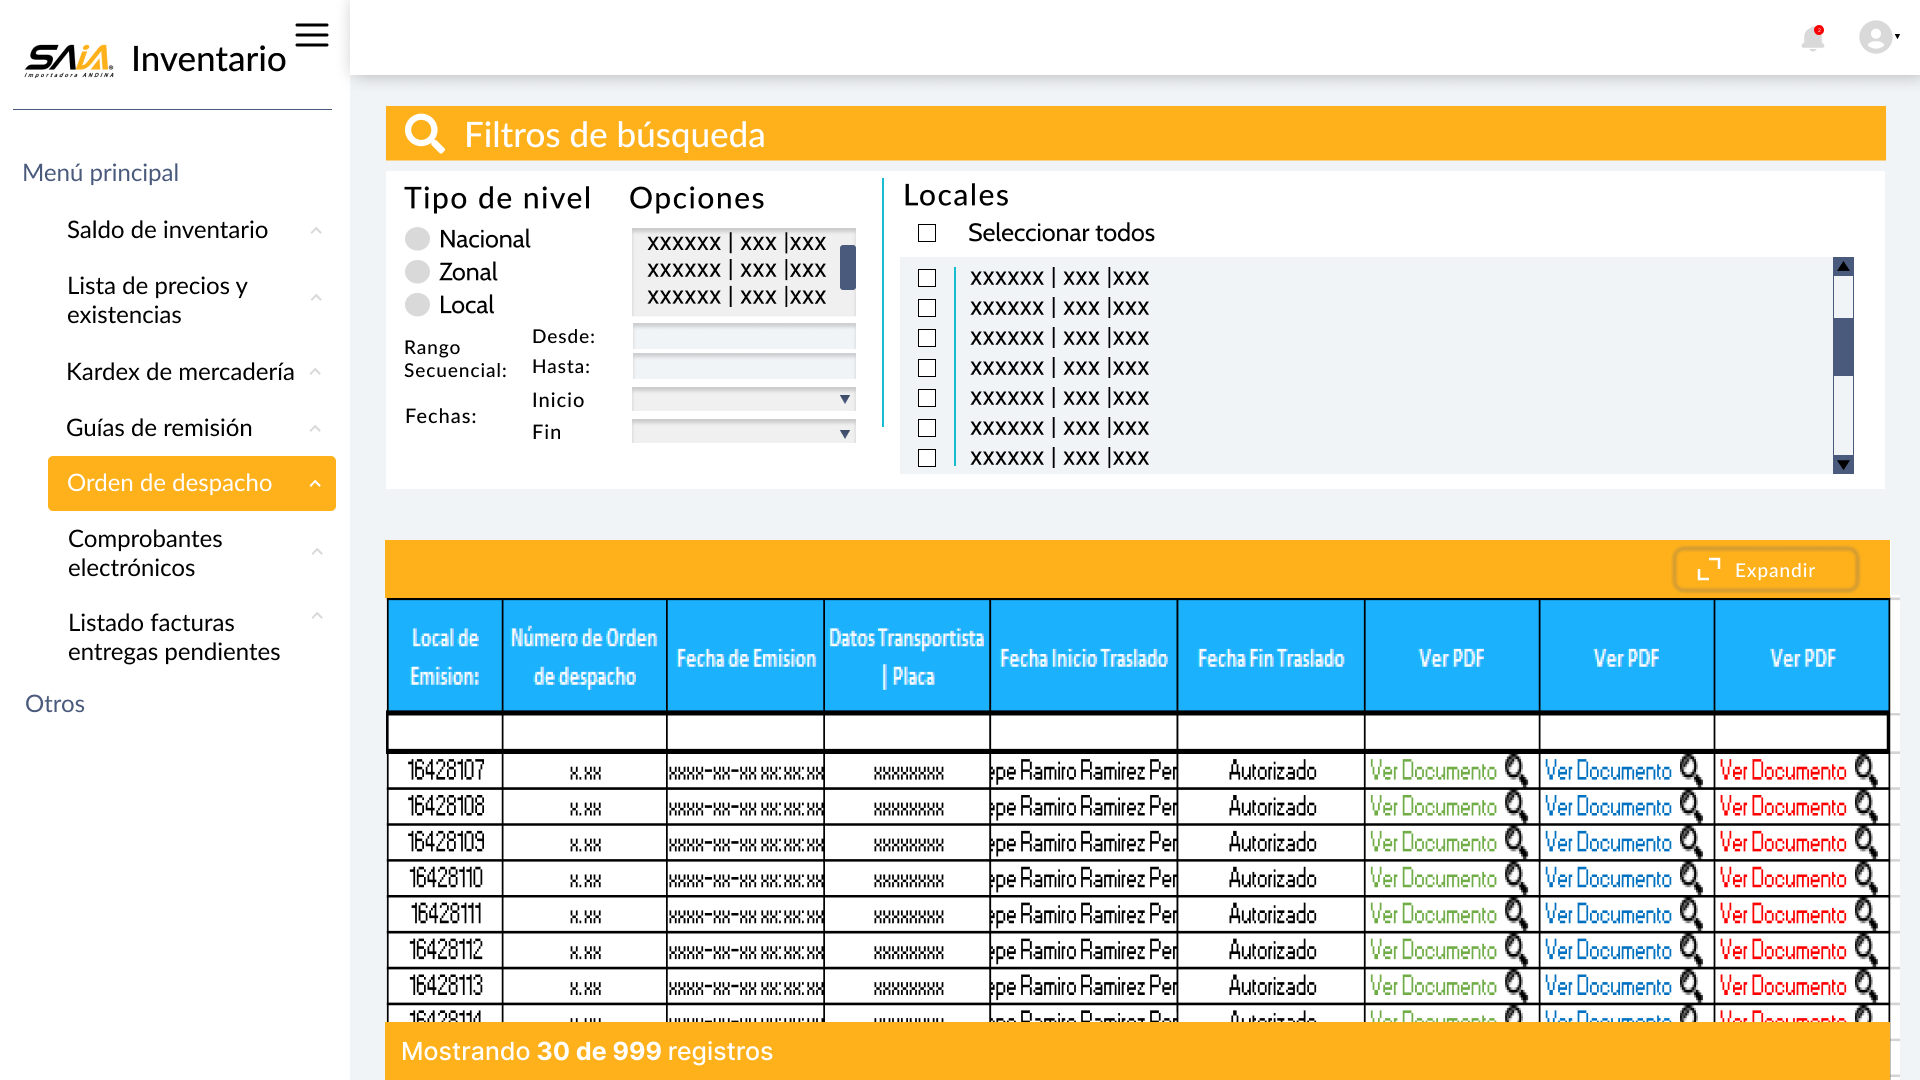
\includegraphics[scale=.22]{images/prototype/web/Ordenes de despacho 2.png}}
        \caption{Resultado de filtros de búsqueda aplicados en Apartado de Ordenes de Despacho.}
        \label{fig}
    \end{figure}
    \FloatBarrier


    \begin{figure}[!htpb]
        \centerline{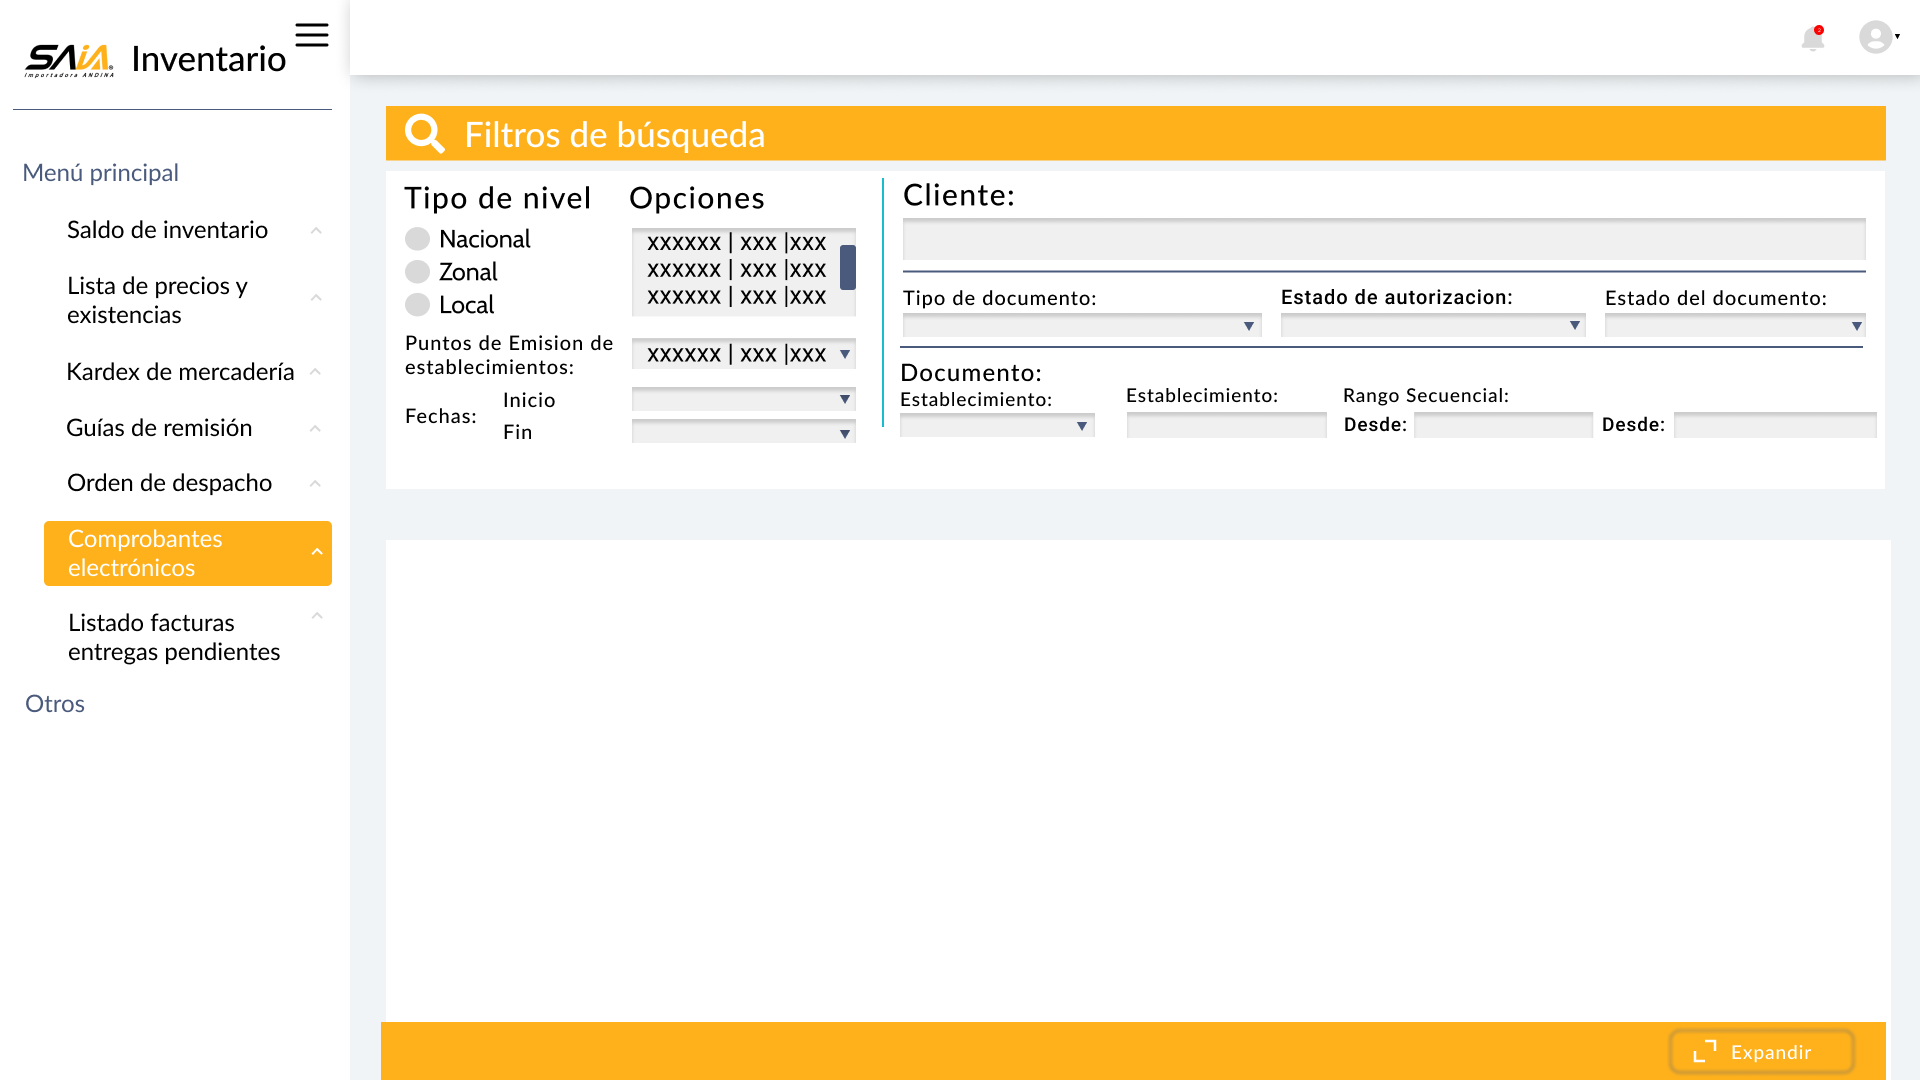
\includegraphics[scale=.22]{images/prototype/web/Comprobantes emitidos.png}}
        \caption{Apartado de Comprobantes Electrónicos.}
        \label{fig}
    \end{figure}
    \FloatBarrier
    \begin{figure}[!htpb]
        \centerline{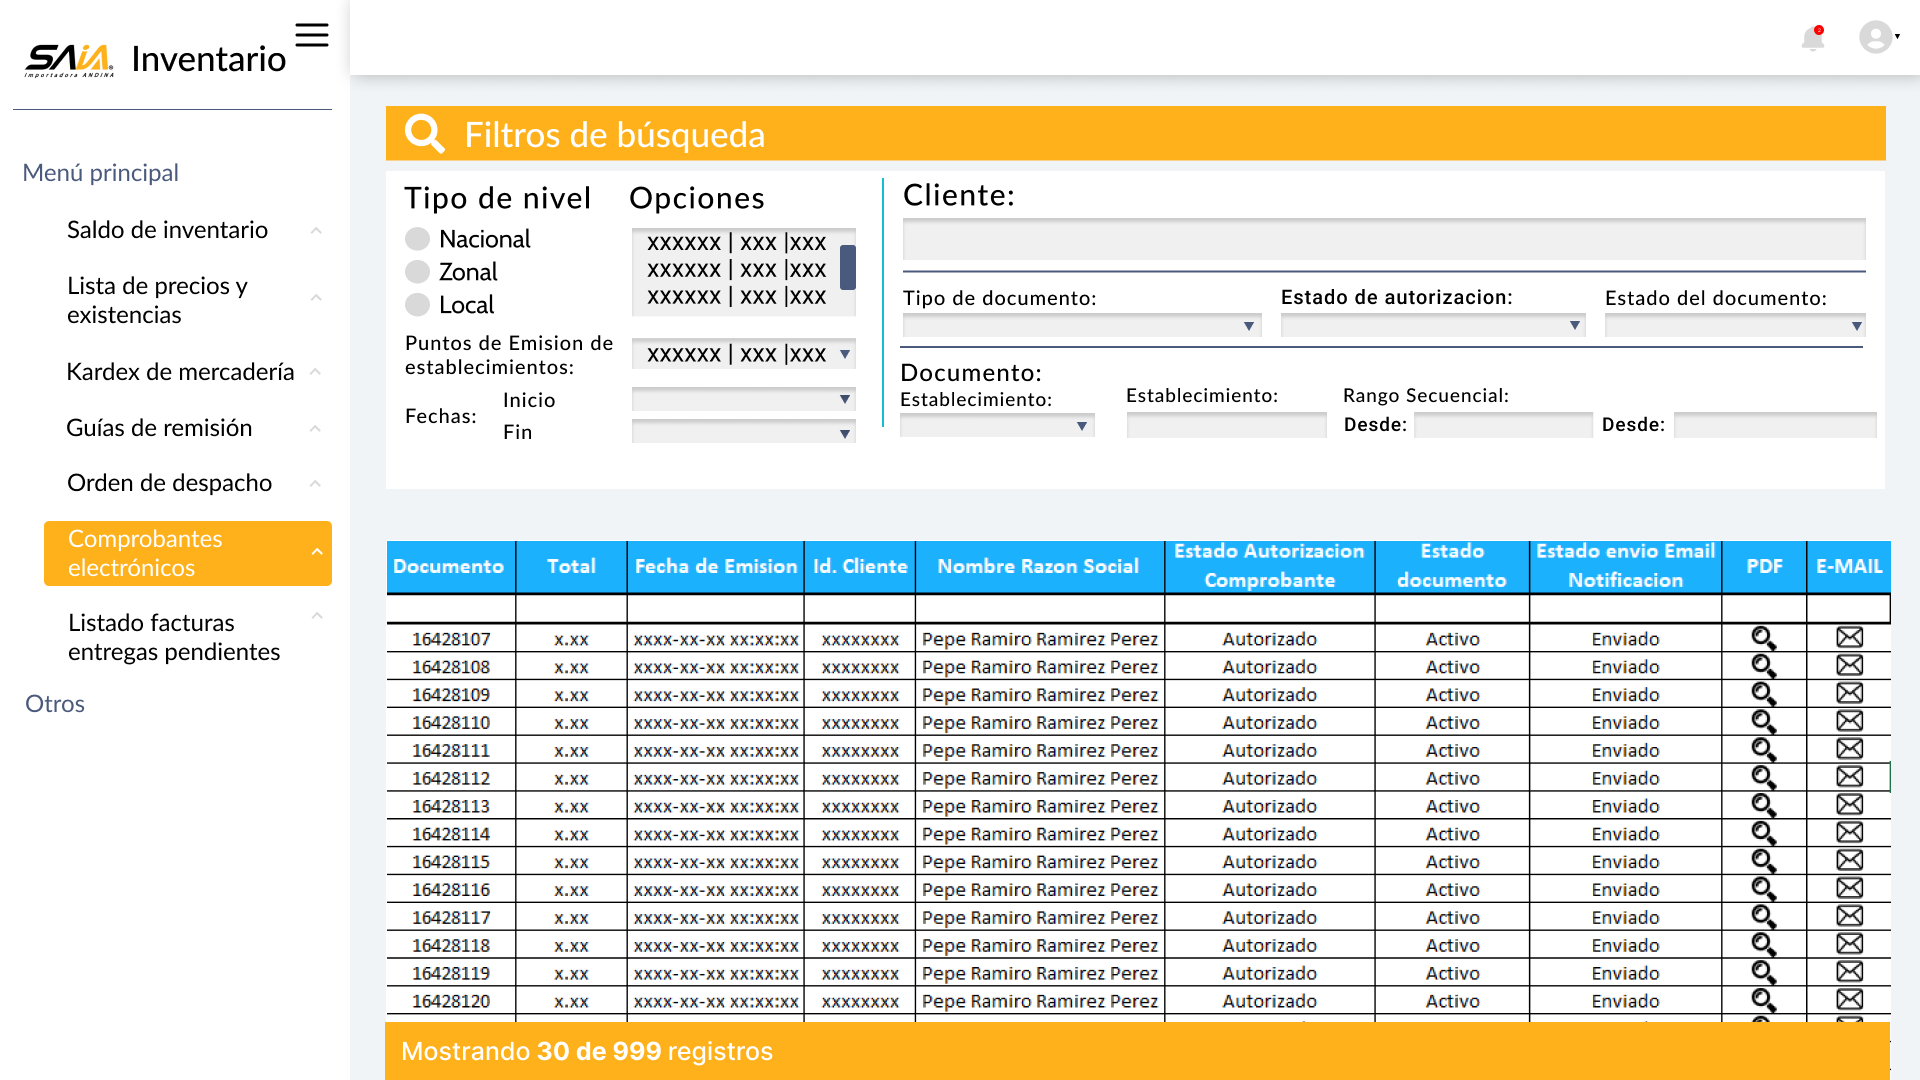
\includegraphics[scale=.22]{images/prototype/web/Comprobantes emitidos 2.png}}
        \caption{Resultado de filtros de búsqueda aplicados en Comprobantes Electrónicos.}
        \label{fig}
    \end{figure}
    \FloatBarrier
    
    
    \begin{figure}[!htpb]
        \centerline{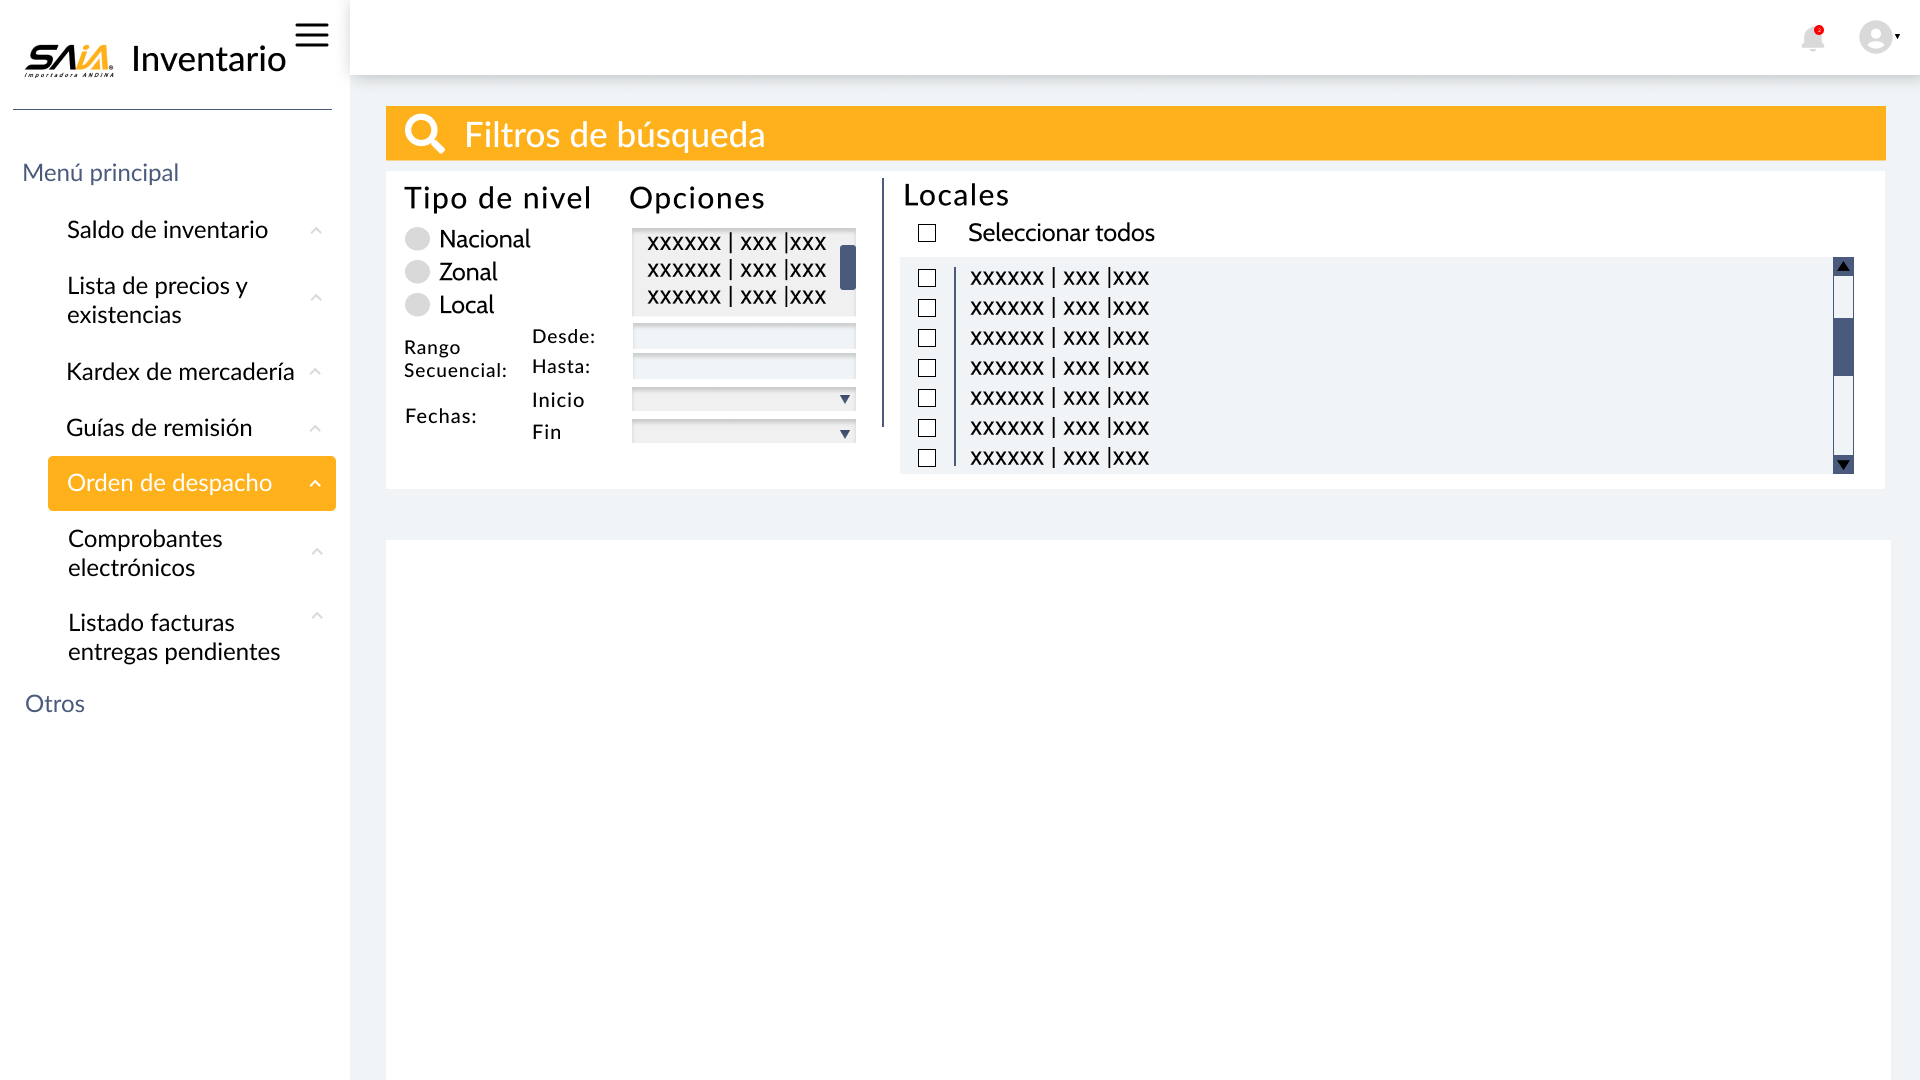
\includegraphics[scale=.22]{images/prototype/web/Ordenes de despacho.png}}
        \caption{Apartado de Ordenes de Despacho.}
        \label{fig}
    \end{figure}
    \FloatBarrier
    \begin{figure}[!htpb]
        \centerline{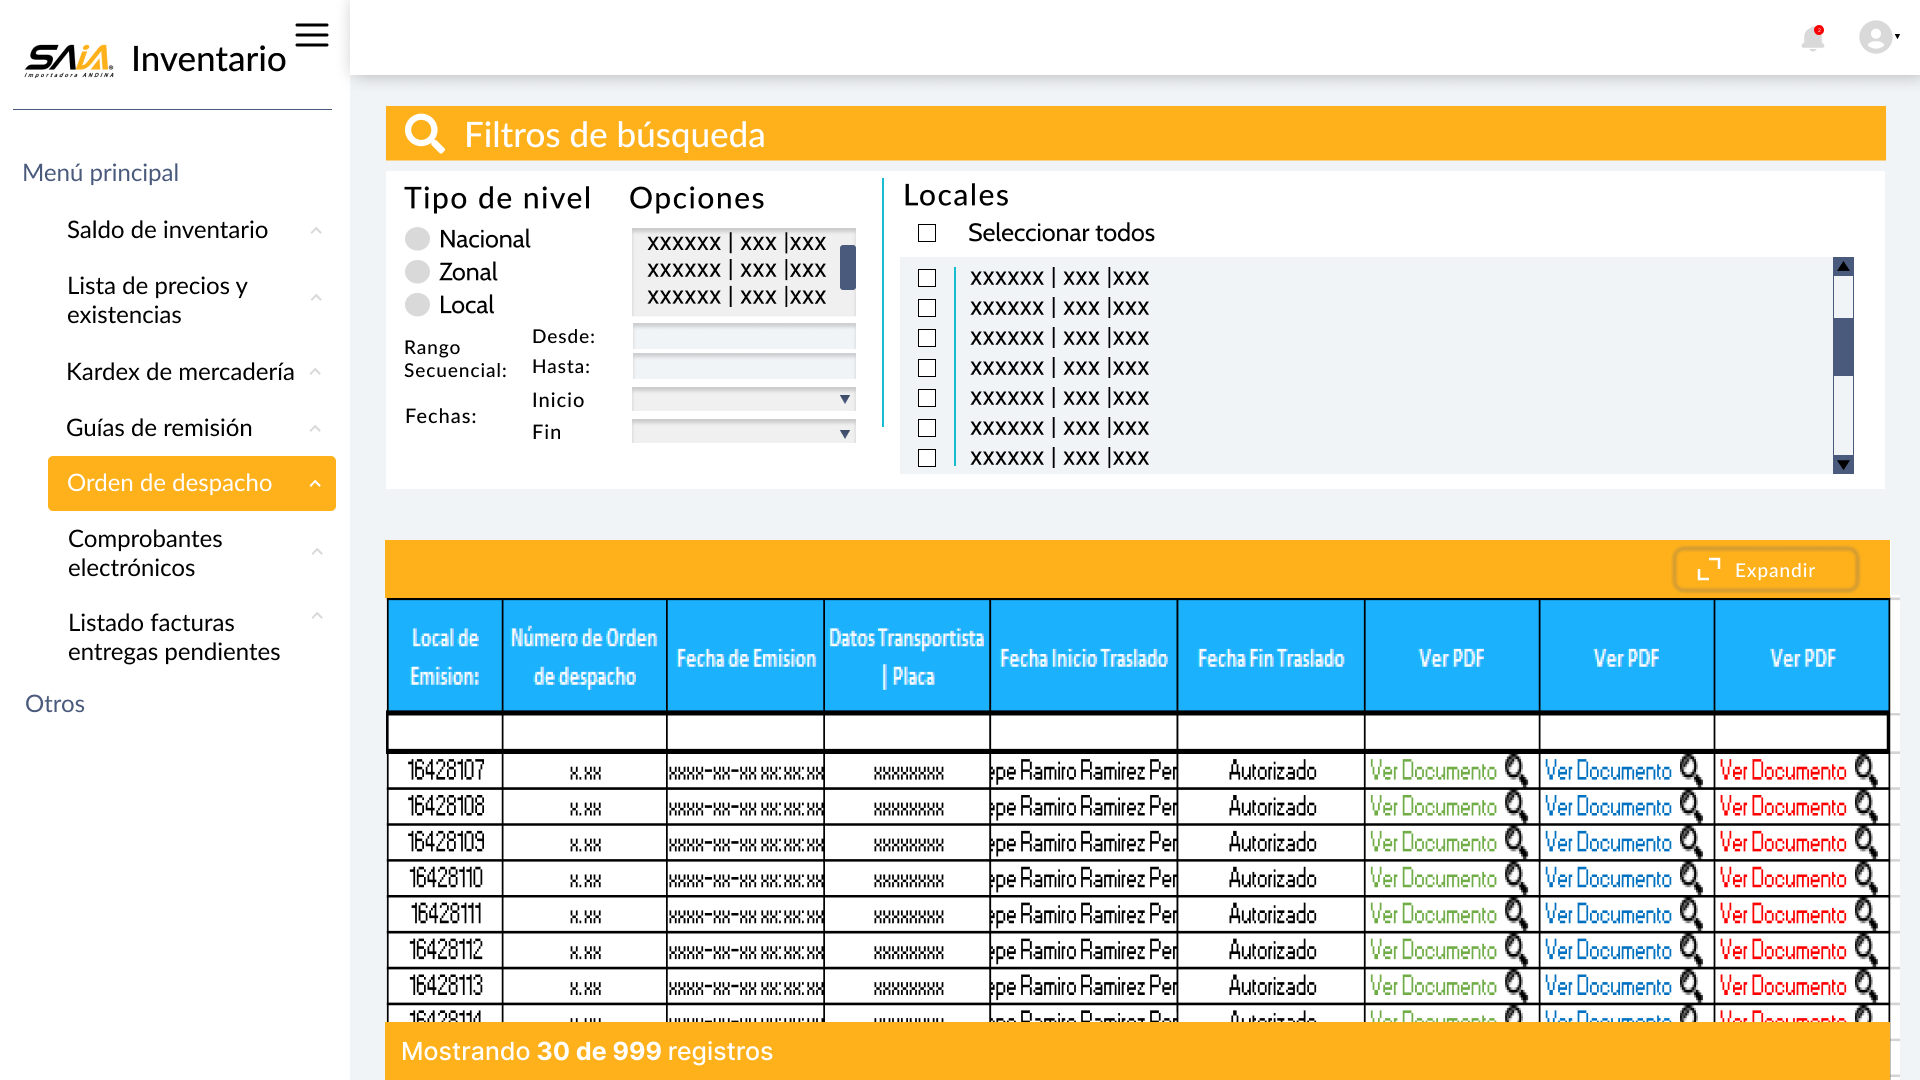
\includegraphics[scale=.22]{images/prototype/web/Ordenes de despacho 2.png}}
        \caption{Resultado de filtros de búsqueda aplicados en Ordenes de Despacho.}
        \label{fig}
    \end{figure}
    \FloatBarrier
    
    
    \begin{figure}[!htpb]
        \centerline{\includegraphics[scale=.22]{images/prototype/web/Guias de remisión.png}}
        \caption{Apartado de Listado de Facturas de Entregas Pendientes.}
        \label{fig}
    \end{figure}
    \FloatBarrier
    \begin{figure}[!htpb]
        \centerline{\includegraphics[scale=.22]{images/prototype/web/Guias de remisión-1.png}}
        \caption{Resultado de filtros de búsqueda aplicados en Listado de Facturas de Entregas Pendientes.}
        \label{fig}
    \end{figure}
    \FloatBarrier
    
    
    \subsection{Aplicativo Móvil}
    
    \begin{figure}[!htpb]
        \centerline{
\includegraphics[scale=.35]{images/prototype/mobile/iPhone 8 - 1.png}}
        \caption{Pantalla de Inicio de Sesión.}
        \label{fig}
    \end{figure}
    \FloatBarrier
    \begin{figure}[!htpb]
        \centerline{
\includegraphics[scale=.35]{images/prototype/mobile/iPhone 8 - 2.png}}
        \caption{Pantalla de Ingreso de Número de Factura.}
        \label{fig}
    \end{figure}
    \FloatBarrier
    \begin{figure}[!htpb]
        \centerline{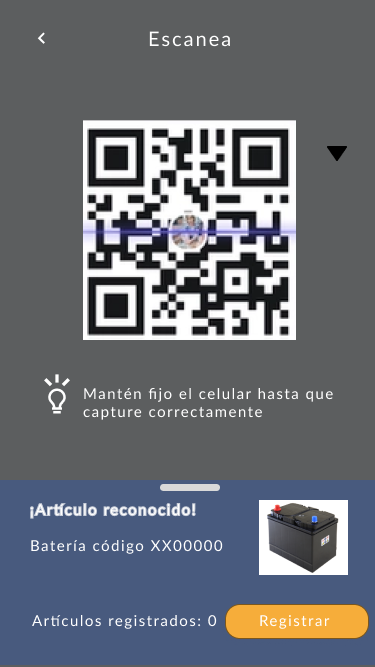
\includegraphics[scale=.35]{images/prototype/mobile/iPhone 8 - 3.png}}
        \caption{Pantalla de Escaneo de Código QR.}
        \label{fig}
    \end{figure}
    \FloatBarrier
    \begin{figure}[!htpb]
        \centerline{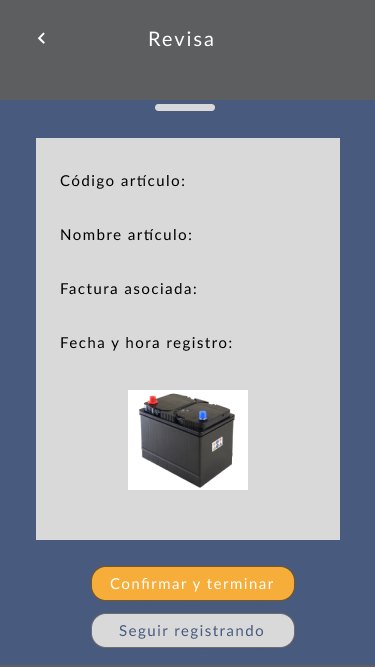
\includegraphics[scale=.35]{images/prototype/mobile/iPhone 8 - 4.png}}
        \caption{Pantalla de Revisión de Información del Producto.}
        \label{fig}
    \end{figure}
    \FloatBarrier
    \begin{figure}[!htpb]
        \centerline{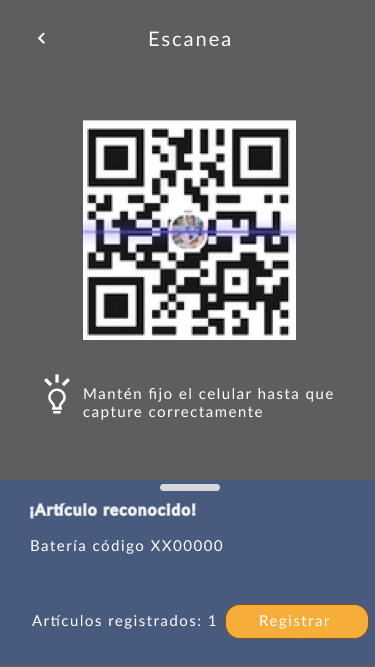
\includegraphics[scale=.35]{images/prototype/mobile/iPhone 8 - 5.png}}
        \caption{Pantalla de Escaneo de Código QR (2).}
        \label{fig}
    \end{figure}
    \FloatBarrier
    \begin{figure}[!htpb]
        \centerline{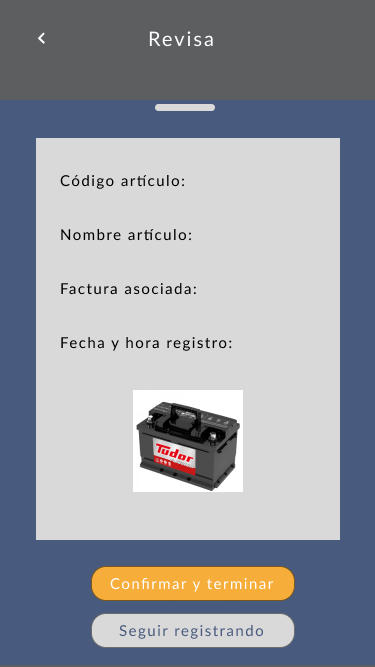
\includegraphics[scale=.35]{images/prototype/mobile/iPhone 8 - 6.png}}
        \caption{Pantalla de Revisión de Información del Producto (2).}
        \label{fig}
    \end{figure}
    \FloatBarrier
    \begin{figure}[!htpb]
        \centerline{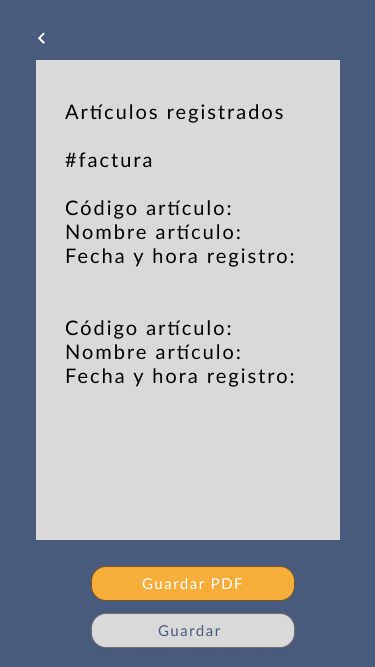
\includegraphics[scale=.35]{images/prototype/mobile/iPhone 8 - 7.png}}
        \caption{Pantalla de Resumen de Productos Registrados.}
        \label{fig}
    \end{figure}
    \FloatBarrier
    \begin{figure}[!htpb]
        \centerline{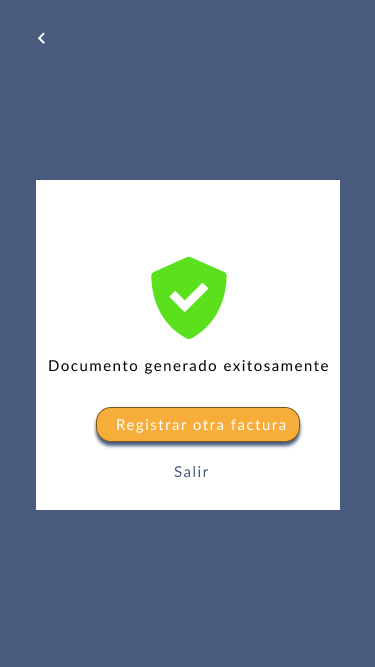
\includegraphics[scale=.35]{images/prototype/mobile/iPhone 8 - 8.png}}
        \caption{Pantalla de Aviso de Documento Generado Correctamente.}
        \label{fig}
    \end{figure}
    \FloatBarrier  

\section{Apéndice D: Firma de Aceptación del Cliente}
    \begin{figure}[ht]
        \centerline{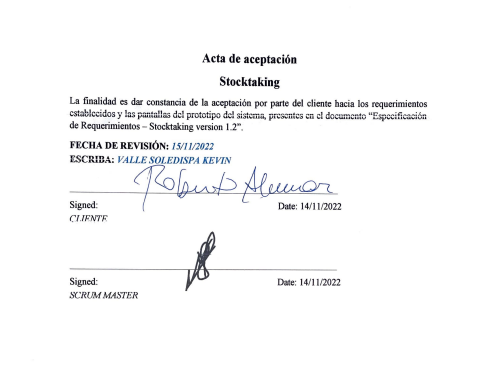
\includegraphics[width=\textwidth]{images/legal_stuff/aceptacion.png}}
    \end{figure}
    \FloatBarrier  
\end{document}